% Dokumentklassen sættes til memoir.
% Manual: http://ctan.org/tex-archive/macros/latex/contrib/memoir/memman.pdf
\documentclass[a4paper,10pt,fleqn]{article}
\usepackage[a4paper]{geometry}
% Danske udtryk (fx figur og tabel) samt dansk orddeling og fonte med

% danske tegn. Hvis LaTeX brokker sig over æ, ø og å skal du udskifte
% "utf8" med "latin1" eller "applemac". 
\usepackage[utf8]{inputenc}
%\usepackage[danish]{babel}
\usepackage[T1]{fontenc}
\usepackage{fixltx2e} 
\usepackage{color}
\usepackage{hyperref}

% Matematisk udtryk, fede symboler, theoremer og fancy ting (fx kædebrøker)
\usepackage{amsmath,amssymb}
\usepackage{stmaryrd}
\usepackage{bm}
\usepackage{amsthm}
\usepackage{tikz}
\usetikzlibrary{arrows}
\usetikzlibrary{positioning}
\usetikzlibrary{snakes}
\usetikzlibrary{decorations.pathreplacing}
\usepackage{mathtools}
\usepackage[makeroom]{cancel}
% Manual: http://mirror.ctan.org/macros/latex/contrib/listings/listings.pdf
\usepackage{listings}
\usepackage{verbatim}
\usepackage{enumitem}
\usepackage{bussproofs}
\usepackage{mathpartir}
 
% Indsættelse af grafik.
\usepackage{graphicx}
\usepackage{xcolor}
\usepackage{multirow}

%\setlength{\mathindent{0cm}}

\newcommand{\sem}[1]{\ensuremath{\llbracket #1 \rrbracket}}
\newcommand{\tuple}[1]{\ensuremath{\langle #1 \rangle}}
\newcommand{\curly}[1]{\ensuremath{\mathcal{#1}}}

\DeclareMathOperator{\FTV}{FTV}
\DeclareMathOperator{\Rel}{Rel}
\DeclareMathOperator{\dom}{dom}
\DeclareMathOperator{\safe}{safe}
\DeclareMathOperator{\irred}{irred}
\DeclareMathOperator{\SNPred}{SN}
\DeclareMathOperator{\val}{Val}
\DeclareMathOperator{\fst}{fst}
\DeclareMathOperator{\snd}{snd}
\DeclareMathOperator{\inl}{inl}
\DeclareMathOperator{\inr}{inr}
\DeclareMathOperator{\scase}{case}
\DeclareMathOperator{\caseof}{of}
\DeclareMathOperator{\fold}{fold}
\DeclareMathOperator{\unfold}{unfold}
\DeclareMathOperator{\epack}{pack}
\DeclareMathOperator{\eunpack}{unpack}
\DeclareMathOperator{\eas}{as}
\DeclareMathOperator{\ein}{in}
\DeclareMathOperator{\enot}{not}

\newcommand{\pack}[3]{\ensuremath{\epack \; \tuple{#1,#2} \; \eas \; #3}}
\newcommand{\unpack}[4]{\ensuremath{\eunpack \; \tuple{#1,#2} = #3 \; \ein \; #4 }}

\newcommand{\evalto}{\ensuremath{\mapsto}}
\newcommand{\evaltos}[1][*]{\ensuremath{\evalto^{#1}}}
\newcommand{\warning}[1]{{\color{red} !` #1 !} \\}
\newcommand{\mtenv}{{\raisebox{1.5pt}{$\scriptstyle\bullet$}}}
\newcommand{\case}[1]{\\{\bf Case} #1,}
\newcommand{\eqdef}{\ensuremath{ \; \stackrel{\mathclap{\normalfont\mbox{def}}}{=} \;}}
\newcommand{\subst}[3]{\ensuremath{\ensuremath{#1[^{\textstyle #2}/_{\textstyle #3}]}}}
\newcommand{\labs}[2]{\ensuremath{\lambda #1 . \; #2}}
\newcommand{\tlabs}[3]{\ensuremath{\lambda #1 : #2 . \; #3}}
\newcommand{\tLabs}[2][\alpha]{\ensuremath{\Lambda #1 . \; #2}}
\newcommand{\vbar}{\ensuremath{\; | \;}}
\newcommand{\tarrow}[2]{\ensuremath{ #1 \rightarrow #2}}
\newcommand{\eif}[3]{\ensuremath{ \text{if}\; #1 \; \text{then} \; #2 \; \text{else} \; #3}}
\newcommand{\true}{\ensuremath{\text{true}}}
\newcommand{\false}{\ensuremath{\text{false}}}
\newcommand{\SN}[2]{\ensuremath{\SNPred_{#1}(#2)}}
\newcommand{\pand}{\ensuremath{\; \wedge \;}}



\newcommand{\pred}[2]{\ensuremath{\curly{#1}\sem{#2}}}
\newcommand{\pres}[3]{\ensuremath{\curly{#1}_{#2}\sem{#3}}}
\newcommand{\prep}[3]{\ensuremath{\curly{#1}\sem{#3}_{#2}}}

\newcommand{\epred}[1]{\pred{E}{#1}}
\newcommand{\epres}[2][k]{\pres{E}{#1}{#2}}
\newcommand{\eprep}[2][\rho]{\prep{E}{#1}{#2}}

\newcommand{\vpred}[1]{\pred{V}{#1}}
\newcommand{\vpres}[2][k]{\pres{V}{#1}{#2}}
\newcommand{\vprep}[2][\rho]{\prep{V}{#1}{#2}}

\newcommand{\gpred}[1]{\pred{G}{#1}}
\newcommand{\gpres}[2][k]{\pres{G}{#1}{#2}}
\newcommand{\gprep}[2][\rho]{\prep{G}{#1}{#2}}

\newcommand{\dpred}[1]{\pred{D}{#1}}

\newcommand{\sub}[3]{\subst{#1}{#2}{#3}}
\newcommand{\extsub}[3]{\ensuremath{#1 \lbrack #2 \mapsto #3 \rbrack}}

\newcommand{\equivalence}[3]{\ensuremath{#1 \approx^{#2} #3}}
\newcommand{\ctxeq}[2]{\equivalence{#1}{ctx}{#2}}
\newcommand{\lreq}[2]{\equivalence{#1}{LR}{#2}}




\newcommand*{\circled}[1]{\tikz[baseline=(char.base)]{
            \node[shape=circle,draw,inner sep=1pt] (char) {#1};}}


\newcommand{\TTrue}{\ensuremath{
    \inferrule*[right=T-True]{ }
               {\Gamma \vdash \true : bool}}}

\newcommand{\TFalse}{\ensuremath{
    \inferrule*[right=T-False]{ }
               {\Gamma \vdash \false : bool}}}
\newcommand{\TVar}{\ensuremath{
    \inferrule*[right=T-Var]{\Gamma(x) = \tau}
                            {\Gamma \vdash x : \tau}}}
\newcommand{\TIf}{\ensuremath{
    \inferrule*[right=T-If]{\Gamma \vdash e : bool \and \Gamma \vdash e_1 : \tau \and \Gamma \vdash e_2 : \tau}
               {\Gamma \vdash \eif{e}{e_1}{e_2} : \tau}}}
\newcommand{\TApp}{\ensuremath{
    \inferrule*[right=T-App]{\Gamma \vdash e_1 : \tarrow{\tau_2}{\tau} \and
                            \Gamma \vdash e_2 : \tau_2}
                           {\Gamma \vdash e_1 \; e_2 : \tau}}}

\newcommand{\TAbs}{\ensuremath{\inferrule*[right=T-Abs]{\Gamma, x: \tau_1 \vdash e : \tau_2}
                           {\Gamma \vdash \tlabs{x}{\tau_1}{e} : \tarrow{\tau_1}{\tau_2}}}}
\newcommand{\TFold}{\ensuremath{
    \inferrule*[right=T-Fold]{\Gamma \vdash e : \tau[\mu\alpha. \; \tau/\alpha]}
                             {\Gamma \vdash \fold \; e : \mu\alpha. \; \tau}}}
\newcommand{\TUnfold}{\ensuremath{
    \inferrule*[right=T-Unfold]{\Gamma \vdash e : \mu\alpha. \; \tau}
                               {\Gamma \vdash \unfold \; e : \tau[\mu\alpha. \; \tau/\alpha]}}}


\newcommand{\FTTrue}{\ensuremath{
    \inferrule*[right=T-True]{ }
               {\Delta ; \Gamma \vdash \true : bool}}}

\newcommand{\FTFalse}{\ensuremath{
    \inferrule*[right=T-False]{ }
               {\Delta ; \Gamma \vdash \false : bool}}}

\newcommand{\FTVar}{\ensuremath{
    \inferrule*[right=T-Var]{\Gamma(x) = \tau}
                            {\Delta ; \Gamma \vdash x : \tau}}}
\newcommand{\FTApp}{\ensuremath{
    \inferrule*[right=T-App]{\Delta ; \Gamma \vdash e_1 : \tarrow{\tau_2}{\tau} \and
                            \Delta ; \Gamma \vdash e_2 : \tau_2}
                           {\Delta ; \Gamma \vdash e_1 \; e_2 : \tau}}}

\newcommand{\FTAbs}{\ensuremath{
    \inferrule*[right=T-Abs]{\Delta ; \Gamma, x: \tau_1 \vdash e : \tau_2}
                           {\Delta ; \Gamma \vdash \tlabs{x}{\tau_1}{e} : \tarrow{\tau_1}{\tau_2}}}}
\newcommand{\FTIf}{\ensuremath{
    \inferrule*[right=T-If]{\Delta ; \Gamma \vdash e : bool \and 
                            \Delta ; \Gamma \vdash e_1 : \tau \\ 
                            \Delta ; \Gamma \vdash e_2 : \tau}
               {\Delta ; \Gamma \vdash \eif{e}{e_1}{e_2} : \tau}}}
\newcommand{\FTtApp}{\ensuremath{
    \inferrule*[right=T-TAbs]{\Delta,\alpha;\Gamma \vdash e : \tau}
                             {\Delta; \Gamma \vdash \tLabs{e} : \forall \alpha.\tau}}}
\newcommand{\FTtAbs}{\ensuremath{
    \inferrule*[right=T-TApp]{\Delta; \Gamma \vdash e : \forall \alpha . \tau \and
                              \Delta \vdash \tau'}
                             {\Delta ; \Gamma \vdash e [\tau'] : \subst{\tau}{\tau'}{\alpha}}}}


\newtheorem*{theorem}{Theorem}
\newtheorem*{lemma}{Lemma}
%Lecture 1:
\newtheorem*{strnorm}{Theorem}
\newtheorem*{astrnorm}{Theorem}
\newtheorem*{substlem}{Lemma}
\newtheorem*{forback}{Lemma}
%Lecture 2:
\newtheorem*{stlctypesafety}{Theorem}
\newtheorem*{progress}{Lemma}
\newtheorem*{preservation}{Lemma}
\newtheorem*{btypesafety}{Theorem}
%Lecture 3:
\newtheorem*{stlcmutypesafety}{Theorem}
\newtheorem*{stlcmufundprop}{Theorem}
\newtheorem*{monotonicity}{Lemma}
%Lecture 4:
\newtheorem*{fundamentalprop}{Theorem}

\author{Lau Skorstengaard\\lask@cs.au.dk}
\title{An Introduction to Logical Predicates and Relations}
\begin{document}
\maketitle This note is based on the lectures of Amal Ahmed at the Oregon Programming Languages Summer School, 2015. The videos of the lectures can be found at \url{https://www.cs.uoregon.edu/research/summerschool/summer15/curriculum.html}. 
\subsection*{Simply Typed Lambda Calculus (STLC)}
The language we use to present logical predicates and relations is the simply typed lambda calculus. In the first section it will be used in its basic form. In the later sections the simply typed lambda calculus will be used as a base language so if it says that we extend with some construct, then it is the simply typed lambda calculus that we extend. The simply typed lambda calculus is defined as follows:\\
\begin{tabular}{ r | l }
  Types: & $\tau ::=  bool \vbar \tarrow{\tau}{\tau}$ \\
  \hline
  Terms: & $e    ::= x \vbar \true 
                       \vbar \false       
                       \vbar \eif{e}{e}{e} 
                       \vbar \tlabs{x}{\tau }{e}
                       \vbar e \; e$ \\
  \hline
  Values: & $v    ::= \true \vbar \false \vbar \tlabs{x}{\tau}{e}$ \\
  \hline
  Evaluation  & \multirow{2}{*}{$E    ::= [] \vbar \eif{E}{e}{e} \vbar E \; e \vbar v \; E$}\\
  contexts: & \\
  \hline
  \multirow{4}{*}{Evaluations:}    
                                   & $\eif{\true}{e_1}{e_2} \evalto e_1$ \\
                                   & $\eif{\false}{e_1}{e_2} \evalto e_2$ \\
                                   & $(\tlabs{x}{\tau}{e}) \; v \evalto \subst{e}{v}{x}$ \\
                                   & $\inferrule*[]{e \evalto e'}
                                                   {E[e] \evalto E[e']}$ \\
  \hline
  Typing & \multirow{2}{*}{$ \Gamma ::= \mtenv \vbar \Gamma , x : \tau$} \\
  Contexts: & \\
  \hline
  \multirow{8}{*}{Typing rules:} & \\
                                 & $\TFalse \hspace{1.2cm} \TTrue$ \\
                                 & \\
                                 & $\TVar \hspace{1.2cm} \TIf$ \\
                                 & \\
                                 & $\TAbs \hspace{1.2cm} \TApp$\\
                                 & \\
\end{tabular}\\
For the typing contexts it is assumed that the binders are distinct. So if $x \in \dom(\Gamma)$, then $\Gamma , x : \tau$ is not a legal context.

\subsection*{Logical Relations}
Logical relations are used to prove properties about programs in a language. Logical relations are proof methods and can be used as an alternative to proving properties directly. Examples of properties one can show using logical relations are:
\begin{itemize}
\item Termination (Strong normalization)
\item Type safety
\item Equivalence of programs
  \begin{itemize}
  \item Correctness of programs
  \item Representation independence
  \item Parametricity and free theorems, e.g.,
    \[
    f: \forall \alpha. \; \tarrow{\alpha}{\alpha}
    \]
    The program cannot inspect $\alpha$ as it has no idea which type it will be, therefore $f$ must be identity function.
    \[
    \forall. \; \tarrow{int}{\alpha}
    \]
    A function with this type does not exist (the function would need to return something of type $\alpha$, but it only has something of type $int$ to work with so it cannot possibly return a value of the proper type).
  \item Security-Typed Languages (for Information Flow Control (IFC))\\
        Example: All types in the code snippet below are labeled with their security level. A type can be labeled with either $L$ for \emph{low} or $H$ for \emph{high}. We do not want any flow from variables with a \emph{high} labeled type to a variable with a \emph{low} labeled type. The following is an example of an insecure \emph{explicit flow} of information:
        \begin{lstlisting}[escapeinside={@}{@}]
  x : int@$^L$@
  y : int@$^H$@
  x = y    //This assignment is insecure.
        \end{lstlisting}
Further, information may leak through a \emph{side channel}. That is the value denoted by a variable with a \emph{low} labeled type depends on the value of a variable with a \emph{high} labeled type. If this is the case we may not have learned the secret value, but we may have learned some information about it. An example of a side channel:
        \begin{lstlisting}[escapeinside={@}{@}]
  x : int@$^L$@
  y : int@$^H$@
  if y > 0 then x = 0 else x = 1
        \end{lstlisting}
The above examples show undesired programs or parts of programs, but if we want to generally state behavior we do not want a program to show, then we state it as non-interference:
\begin{align*}
  & \vdash P : \tarrow{int^L \times int^H}{int^L} \\
  & P(v_L,v_{1H}) \approx_L P(v_L,v_{2H})
\end{align*}
If we run $P$ with the same \emph{low} value and with two different \emph{high} values, then the \emph{low} result of the two runs of the program should be equal. That is the \emph{low} result does not depend on \emph{high} values.
  \end{itemize}
\end{itemize}
\subsection*{Categories of Logical Relations}
We can split logical relations into two logical relations and logical predicates. Logical predicates are unary and used usually used to show properties of a program. Logical relations are binary and are usually used to show equivalences:\\
\begin{tabular}{l | l}
  Logical Predicates     & Logical Relations    \\
\hline
  (Unary)                & (Binary)             \\
  $P_\tau(e)$             & $R_\tau(e_1,e_2)$     \\
  - One property         & - Program Equivalence\\ %\footnote{Was not in my notes.}
  - Strong normalization & \\
  - Type safety          & \\
\end{tabular}
The following describes some properties we in general want a logical \emph{predicate} to have. These properties can be generalized to logical relations.

In general for a logical predicate, $P_\tau(e)$, we want an expression, $e$, accepted by this predicate to satisfy the following properties\footnote{Note: when we later want to prove type safety the well-typedness property is weakened to only require $e$ to be closed.}:
\begin{enumerate}
\item $\mtenv \vdash e : \tau$
\item The property we wish $e$ to have. In this case it would be: $e$ is strongly normalizing.
\item The condition is preserved by eliminating forms.
\end{enumerate}

\section*{Normalization of the Simply Typed Lambda Calculus}
\subsection*{Strong Normalization of STLC}
In this section we wish to show that the simply typed lambda calculus has strong normalization which means that every term is strongly normalizing. Normalization of a term is the process of reducing a term into its normal form. If a term is strongly normalizing, then it reduces to its normal form. In our case we define the normal forms of the language to be the values of the language.
\subsubsection*{A first try on normalization of STLC}
We start with a couple of abbreviations:
\begin{align*}
  e \Downarrow v & \eqdef e \evaltos v \\
  e \Downarrow   & \eqdef \exists v. \; e \Downarrow v
\end{align*}
Where $v$ is a value.
What we want to prove is:
\begin{strnorm}[Strong Normalization]~\\
  If $\mtenv \vdash e : \tau$ then $e \Downarrow$
\end{strnorm}
We first try to prove the above property directly to see it fail.
\begin{proof} 
\warning{This proof gets stuck and is not complete.}
Induction on the structure of the typing derivation.
\case{$\mtenv \vdash \true : bool$} this term has already terminated.
\case{$\mtenv \vdash \false : bool$} same as for \true.
\case{$\mtenv \vdash \eif{e}{e_1}{e_2} : \tau$} simple, but requires the use of canonical forms of bool.
\case{$\mtenv \vdash \tlabs{x}{\tau_1}{e}$ : \tarrow{\tau_1}{\tau_2}} it is a value already and it has terminated.
\case{$ \TApp $} \\
By the induction hypothesis we get $e_1 \Downarrow v_1$ and $e_2 \Downarrow v_2$. By the type of $e_1$ we conclude $e_1 \Downarrow \tlabs{x}{\tau_2}{e'}$. What we need to show is $e_1 \; e_2 \Downarrow$. We know $e_1 \; e_2$ takes the following steps:
\begin{align*}
  e_1 \; e_2 & \evaltos (\tlabs{x}{\tau_2}{e'}) \; e_2 \\
            & \evaltos (\tlabs{x}{\tau_2}{e'}) \; v_2 \\
            & \evalto e'[v_2/x]
\end{align*}
Here we run into an issue as we do not know anything about $e'$. Our induction hypothesis is not strong enough.\footnote{:(}
\end{proof}

\subsubsection*{A logical predicate for strongly normalizing expressions}
We want to define a logical predicate, \SN{\tau}{e}. We want $\SNPred_\tau$ to accept the expressions of type $\tau$ that are strongly normalizing. In the introduction we considered some properties a logical predicate in general predicate should have. Keep these properties in mind when we define the logical predicate for strong normalization:
\begin{align*}
  \SN{bool}{e} & \Leftrightarrow \mtenv \vdash e : bool \pand e \Downarrow \\
  \SN{\tarrow{\tau_1}{\tau_2}}{e} & \Leftrightarrow \mtenv \vdash e : \tarrow{\tau_1}{\tau_2} \pand e \Downarrow \pand (\forall e'. \; \SN{\tau_1}{e'} \implies \SN{\tau_2}{e \; e'})\\
\end{align*}
It is here important to consider whether the logical predicate is well-founded. \SN{\tau}{e} is defined over the structure of $\tau$, so it is indeed well-founded.
\subsubsection*{Strongly normalizing using a logical predicate}
We are now ready to show strong normalization using \SN{\tau}{e}. The proof is done in two steps:
\[
\circled{a} \quad \mtenv \vdash e : \tau \implies \SN{\tau}{e}
\]
\[
\circled{b} \quad \SN{\tau}{e} \implies e \Downarrow
\]
The structure of this proof is common to proofs that use logical relations. We first prove that well-typed terms are in the relation. Then we prove that terms in the relation actually have the property we want to show (in this case strong normalization).

The proof of \circled{b} is by induction on $\tau$.\footnote{This should not be difficult, as we baked the property we want into the relation. That was the second property we in general wanted a logical relation to satisfy.}

We could try to prove \circled{a} by induction over $\mtenv \vdash e : \tau$, but the case
\[
  \TAbs
\]
gives issues. Instead we prove a generalization of \circled{a}
\begin{astrnorm}[\circled{a} Generalized]
  If $\Gamma \vdash e : \tau$ and $\gamma \models \Gamma$ then $\SN{\tau}{\gamma(e)}$
\end{astrnorm}
Here $\gamma$ is a substitution, $\gamma = \{x_1 \mapsto v_1, \dots , x_n \mapsto v_n\}$. We define the substitution to work as follows:
\begin{align*}
  & \emptyset (e) = e \\
  & \extsub{\gamma}{x}{v}(e) = \gamma(\subst{e}{x}{v})
\end{align*}

In English the theorem reads: If $e$ is well-typed with respect to some type $\tau$ and we have some closing substitution that satisfy the typing environment, then if we close of $e$ with $\gamma$, then this closed expression is in $\SNPred_\tau$.

$\gamma \models \Gamma$ is read ``the substitution, $\gamma$, satisfies the type environment, $\Gamma$.'' It is defined as follows:
\[
  \gamma \models \Gamma \eqdef \dom(\gamma) = \dom(\Gamma) \pand 
                 \forall x \in \dom(\Gamma). \; \SN{\Gamma(x)}{\gamma(x)}
\]
To prove the generalized theorem we need further two lemmas
\begin{substlem}[Substitution Lemma]
  If $\Gamma \vdash e : \tau$ and $\gamma \models \Gamma$ then $\mtenv \vdash \gamma (e) : \tau$
\end{substlem}
\begin{forback}[$\SNPred$ preserved by forward/backward reduction]
  Suppose $\mtenv \vdash e : \tau$ and $e \evalto e'$
  \begin{enumerate}
  \item if $\SN{\tau}{e'}$ then $\SN{\tau}{e}$
  \item if $\SN{\tau}{e}$ then $\SN{\tau}{e'}$
  \end{enumerate}
\end{forback}
\begin{proof}
  Probably also left as an exercise (not proved during the lecture).
\end{proof}
\begin{proof}[Proof. (Substitution Lemma)] 
  Left as an exercise.
\end{proof}
\begin{proof}[Proof. (\circled{a} Generalized)] Proof by induction on $\Gamma \vdash e : \tau$.
\case{$\Gamma \vdash \true : bool$} \\
We have: 
\begin{description}
  \item $\gamma \models \Gamma$
\end{description}
We need to show:
\begin{description}
  \item $\SN{bool}{\gamma(\true)}$
\end{description}
If we do the substitution we just need to show $\SN{bool}{\true}$ which is true by definition of $\SN{bool}{\true}$.
\case{$\Gamma \vdash \false : bool$} similar to the \true{} case.
\case{\TVar}\\
We have: 
\begin{description}
  \item $\gamma \models \Gamma$
\end{description}
We need to show:
\begin{description}
  \item $\SN{\tau}{\gamma(x)}$
\end{description}
This case follows from the definition of $\Gamma \models \gamma$. We know that $x$ is well-typed, so it is in the domain of $\Gamma$. From the definition of $\Gamma \models \gamma$ we then get $\SN{\Gamma(x)}{\gamma(x)}$. From well-typedness of $x$ we have $\Gamma(x) = \tau$ which then gives us what we needed to show.
\case{$\Gamma \vdash \eif{e}{e_1}{e_2} : \tau$} left as an exercise.
\case{\TApp}\\
We have: 
\begin{description}
  \item $\gamma \models \Gamma$
\end{description}
We need to show:
\begin{description}
  \item $\SN{\tau}{\gamma(e_1 \; e_2)} \equiv \SN{\tau}{\gamma(e_1) \; \gamma(e_2)}$
\end{description}
By the induction hypothesis we have
\begin{align}
  &\SN{\tarrow{\tau_2}{\tau}}{\gamma(e_1)} \\
  &\SN{\tau_2}{\gamma(e_2)}
\end{align}
If we use the 3rd property of (1), $\forall e'. \; \SN{\tau_2}{e'} \implies \SN{\tau}{\gamma(e_1) \; e'}$, instantiated with (2), then we get $\SN{\tau}{\gamma(e_1) \; \gamma(e_2)}$ which is the result we need.
\case{\TAbs} \\
We have: 
\begin{description}
  \item $\gamma \models \Gamma$
\end{description}
We need to show:
\begin{description}
  \item $\SN{\tarrow{\tau_1}{\tau_2}}{\gamma(\tlabs{x}{\tau_1}{e})} \equiv \SN{\tarrow{\tau_1}{\tau_2}}{\tlabs{x}{\tau_1}{\gamma(e)}}$
\end{description}
Our induction hypothesis in this case reads:
\[
  \Gamma,x:\tau_1 \vdash e : \tau_2 \pand \gamma' \models \Gamma, x : \tau_1 \quad \implies \quad \SN{\tau_2}{\gamma'(e)}
\]
It suffices to show the following three things:
\begin{enumerate}
\item $\mtenv \vdash \tlabs{x}{\tau_1}{\gamma(e)} : \tarrow{\tau_1}{\tau_2}$
\item $\tlabs{x}{\tau_1}{\gamma(e)} \Downarrow$
\item $\forall e'. \SN{\tau_1}{e'} \implies \SN{\tau_2}{(\tlabs{x}{\tau_1}{\gamma(e)}) \; e'}$
\end{enumerate}
If we use the substitution lemma and push the $\gamma$ in under the $\lambda$-abstraction, then we get 1\footnote{Substitution has not been formally defined here, but one can find a sound definition in Pierce's Types and Programming Languages.}. 2 is okay as the lambda-abstraction is a value. 

It only remains to show 3. To do this we want to somehow apply the induction hypothesis for which we need a $\gamma'$ such that $\gamma' \models \Gamma, x:\tau_1$. We already have $\gamma$ and $\gamma \models \Gamma$, so our $\gamma'$ should probably have have the form $\gamma' = \gamma[x \mapsto v_?]$ for some $v_?$ of type $\tau_1$. Let us move on and see if any good candidates for $v_?$ present themselves.

Let $e'$ be given and assume $\SN{\tau_1}{e'}$. We then need to show $\SN{\tau_2}{(\tlabs{x}{\tau_1}{\gamma(e)}) \; e'}$. From $\SN{\tau_1}{e'}$ it follows that $e' \Downarrow v'$ for some $v'$. $v'$ is a good candidate for $v_?$ so let $v_? = v'$. From the forward part of the preservation lemma we can further conclude $\SN{\tau_1}{v'}$. We use this to conclude $\gamma[x\mapsto v'] \models \Gamma, x:\tau_1$ which we use with the assumption $\Gamma,x:\tau_1 \vdash e : \tau_2$ to instantiate the induction hypothesis and get $\SN{\tau_2}{\gamma[x\mapsto v'](e)}$.

Now consider the following evaluation:
\begin{align*}
  (\tlabs{x}{\tau_1}{\gamma(e)}) \; e' & \evaltos (\tlabs{x}{\tau_1}{\gamma(e)}) \; v' \\
                                       & \evalto \gamma(e)[v'/x] \equiv 
                                                   \gamma[x \mapsto v'](e)
\end{align*}
We already concluded that $e' \evaltos v'$ which corresponds to the first series of steps. We can then do a $\beta$-reduction to take the next step and finally we get something that is equivalent to $\gamma[x \mapsto v'](e)$. That is we have the evaluation
\[
(\tlabs{x}{\tau_1}{\gamma(e)}) \; e' \evaltos \gamma[x \mapsto v'](e)
\]
From \SN{\tau_1}{e'} we have $\mtenv \vdash e' : \tau_1$ and we already argued that $\mtenv \vdash \tlabs{x}{\tau_1}{\gamma(e)} : \tarrow{\tau_1}{\tau_2}$ so from the application typing rule we get $\mtenv \vdash (\tlabs{x}{\tau_1}{\gamma(e)}) \; e' : \tau_2$. We can use this with the above evaluation and the forward part of the preservation lemma to argue that every intermediate expressions in the steps down to $\gamma[x \mapsto v'](e)$ are closed and well typed.

If we use \SN{\tau_2}{\gamma[x\mapsto v'](e)} with $(\tlabs{x}{\tau_1}{\gamma(e)}) \; e' \evaltos \gamma[x \mapsto v'](e)$ and the fact that every intermediate step in the evaluation is closed and well typed, then we can use the backward reduction part of the $\SNPred$ preservation lemma to get \SN{\tau_2}{(\tlabs{x}{\tau_1}{\gamma(e)}) \; e'} which is the result we wanted.
\end{proof}
\subsection*{Exercises}
\begin{enumerate}
\item Prove $\SNPred$ preserved by forward/backward reduction.
\item Prove the substitution lemma.
\item Go through the cases of ``\circled{a} Generalized'' shown here by yourself.
\item Prove the if-case of ``\circled{a} Generalized''.
\item Extend the language with pairs and do the proofs. 
  \begin{enumerate}
  \item See how the clauses, we generally wanted our logical predicate to have, play out when we extend the logical predicate. Do we need to add anything for the third clause or does it work out without putting anything there like we did with the $bool$ case.
  \end{enumerate}
\end{enumerate}
\clearpage

First we need to consider what type safety is. The classical mantra for type safety is ``Well-typed programs do not \emph{go wrong}.'' It depends on the language and type system what \emph{go wrong} means, but in our case a program has \emph{gone wrong} if it is stuck\footnote{If we consider language-based security for information flow control the notion of \emph{go wrong} would be that there is an undesired flow of information} (an expression is stuck if it is irreducible but not a value). 

\section*{Type Safety for STLC}
In the following section we want to prove type safety for the simply typed lambda calculus. We do not want to prove it directly as one normally does. We want to prove it using a logical predicate.

First we need to consider what type safety is. The classical mantra for type safety is ``Well-typed programs do not \emph{go wrong}.'' It depends on the language and type system what \emph{go wrong} means, but in our case a program has \emph{gone wrong} if it is stuck\footnote{If we consider language-based security for information flow control the notion of \emph{go wrong} would be that there is an undesired flow of information} (an expression is stuck if it is irreducible but not a value). 
\subsection*{Type safety - the classical treatment}
Type safety for simply typed lambda calculus is stated as follows:
\begin{stlctypesafety}[Type Safety for STLC]
  If $\mtenv \vdash e : \tau$ and $e \evaltos e'$ then $\val(e')$ or $\exists e''. \; e' \evalto e''$.
\end{stlctypesafety}
Traditionally type safety is proven with two lemmas, progress and preservation.
\begin{progress}[Progress]
  If $\mtenv \vdash e : \tau$ then $\val(e)$ or $\exists e'. \; e \evalto e'$.
\end{progress}
Progress is normally proved by induction on the typing derivation.
\begin{preservation}[Preservation]
  If $\mtenv \vdash e : \tau$ and $e \evalto e'$ then $\mtenv \vdash e' : \tau$.
\end{preservation}
Preservation is normally proved by induction on the evaluation.
Preservation is also known as \emph{subject reduction}. Progress and preservation talk about one step, so to prove type safety we have to do induction on the evaluation. Here we do not want to prove type safety the traditional way. We want to prove it using a logical predicate. We use a logical predicate rather than a logical relation because type safety is a unary property.

\subsection*{Type safety - using logical predicate}
The notation will here be changed compared to the one from lecture 1. We define the logical predicate in two parts: a value interpretation and an expression interpretation. The value interpretation is a function from types to the power set of closed values:
\[
  \vpred{ } : \tarrow{type}{\curly{P}(ClosedVal)}
\]
The value interpretation is defined as:
\begin{align*}
  \vpred{bool} & = \{ \true, \false \}\\
  \vpred{\tarrow{\tau_1}{\tau_2}} & = \{\tlabs{x}{\tau_1}{e} \vbar \forall v \in \curly{V}\sem{\tau_1}.\; e [v/x] \in \curly{E}\sem{\tau_2}\}
\end{align*}
We define the expression interpretation as:
\[
  \epred{\tau} = \{e \vbar \forall e'. \; e \evaltos e' \pand \irred(e') \implies e' \in \curly{V}\sem{\tau} \}
\]
\footnote{Notice that neither \vpred{\tau} nor \epred{\tau} requires well-typedness. Normally this would be a part of the predicate, but as the goal is to prove type safety we do not want it as a part of the predicate. In fact, if we did include a well-typedness requirement, then we would end up having to prove preservation for some of the proofs to go through. We do, however, require the value interpretation to only contain closed values.}The predicate $\irred$ is defined as:
\[
  \irred(e) \eqdef \not\exists e'. \; e \evalto e'
\]
%TODO: Exlpain in words what irred is.
The sets are defined on the structure of the types. \vpred{\tarrow{\tau_1}{\tau_2}} contains \epred{\tau_2}, but \epred{\tau_2} uses $\tau_2$ directly in \vpred{\tau_2}, so the definition is structurally well-founded. To prove type safety we first define a new predicate, $\safe$:
\[
  \safe(e) \eqdef \forall e' . \; e \evaltos e' \implies \val(e') \vee \exists e
''. \; e' \evaltos e''
\]
%TODO: Explain in words what safe is
We are now ready to prove type safety. Just like we did for strong normalization, we prove type safety in two steps:
\[
  \circled{a} \quad \mtenv \vdash e : \tau \implies e \in \epred{\tau}
\]
\[
  \circled{b} \quad e \in \epred{\tau} \implies \safe(e)
\]
Rather than proving \circled{a} directly we prove a more general theorem and get \circled{a} as a corollary. But we are not yet in a position to state the theorem. First we need to define define the interpretation of type environments:
\begin{align*}
  \gpred{\mtenv} & = \{ \emptyset \} \\
  \gpred{\Gamma,x:\tau} & = \{\gamma[x \mapsto v] \vbar 
    \gamma \in \gpred{\Gamma} \pand 
    v \in \vpred{\tau}\}
\end{align*}
Further we need to define semantic type safety:
\[
  \Gamma \models e : \tau \eqdef \forall \gamma \in \gpred{\Gamma} . \; \gamma(e) \in \epred{\tau}
\]
We can now define our generalized version of \circled{a}. 
\begin{btypesafety}[Fundamental Property]
  If $\Gamma \vdash e : \tau$ then $\Gamma \models e : \tau$
\end{btypesafety}
A theorem like this would typically be the first you prove after defining a logical relation. The theorem says that every syntactic type safety implies semantic type safety. 

We also alter the \circled{b} part of the proof, so we prove
\[
  \mtenv \models e : \tau \implies \safe(e)
\]
\begin{proof}[Proof. (Altered \circled{b})]
Suppose $e \evaltos e'$ for some $e'$, then we need to show $\val(e')$ or $\exists e''. \; e' \evalto e''$. We proceed by casing on whether or not $\irred(e')$:
\case{$\neg \irred(e')$} this case follows directly from the definition of $\irred$. $\irred(e')$ is defined as $\not \exists e''. \; e' \evalto e''$ and as the assumption is $\neg \irred(e')$ we get $\exists e''. \; e' \evalto e''$.
\case{$\irred(e')$} By assumption we have $\mtenv \models e : \tau$. As the typing context is empty we choose the empty substitution and get $e \in \epred{\tau}$. We now use the definition of $e \in \epred{\tau}$ with what we supposed, $e \evaltos e'$, and the case assumption, $\irred(e')$, to conclude $e' \in \vpred{\tau}$. As $e'$ is in the value interpretation of $\tau$ we can conclude $\val(e')$. 
\end{proof}
To prove the Fundamental Property we need a substitution lemma:
\begin{lemma}[Substitution]
Let $e$ be syntactically well-formed term, let $v$ be a closed value and let $\gamma$ be a substitution that map term variables to closed values, and let $x$ be a variable not in the domain of $\gamma$, then
\[
\extsub{\gamma}{x}{v}(e) = \subst{\gamma(e)}{x}{v}
\]
\end{lemma}
\begin{proof}
  By induction on the size of $\gamma$.
  \case{$\gamma = \emptyset$} This case is immediate by how substitution is defined. That is by definition we have $[x \mapsto v] e = \subst{e}{v}{x}$.
  \case{$\gamma = \gamma'[y \mapsto v']$, $x\neq y$} In this case our induction hypothesis is:
\[
  \gamma'[x \mapsto v] e = \subst{\gamma'(e)}{v}{x}
\]
We wish to show 
\[
  \gamma'[y \mapsto v'][x \mapsto v] e = \subst{\gamma'[y \mapsto v'](e)}{v}{x}
\]
\begin{align}
    \gamma'[y \mapsto v'][x \mapsto v] e & = \gamma'[x \mapsto v][y \mapsto v'] e \label{sub:step1}\\
                                         & = \gamma'[x \mapsto v] (\subst{e}{v'}{y}) \label{sub:step2}\\
                                         & = \subst{\gamma'(\subst{e}{v'}{y})}{x}{v}\label{sub:step3}\\
                                         & = \subst{\gamma'[y \mapsto v'](e)}{x}{v}\label{sub:step4}
\end{align}
In the first step (\ref{sub:step1}) we swap the two mappings. It is safe to do so as both $v$ and $v'$ are closed so we know that no variable capturing will occur. In the second step (\ref{sub:step2}) we just use the definition of substitution (as specified in the first lecture note). In third step (\ref{sub:step3}) we use the induction hypothesis\footnote{The induction hypothesis actually has a number of premises, as an exercise convince yourself that they are satisfied.}. Finally in the last step (\ref{sub:step4}) we use the definition of substitution to get the $y$ binding out as an extension of $\gamma'$.
\end{proof}
\begin{proof}[Proof. (Fundamental Property)] Proof by induction on the typing judgment.
  \case{\TAbs} \\
We need to show $\Gamma \models \tlabs{x}{\tau_1}{e} : \tarrow{\tau_1}{\tau_2}$. First suppose $\gamma \in \gpred{\Gamma}$. Then we need to to show
\[
  \gamma(\tlabs{x}{\tau_1}{e}) \in \epred{\tarrow{\tau_1}{\tau_2}} \equiv
  (\tlabs{x}{\tau_1}{\gamma(e)}) \in \epred{\tarrow{\tau_1}{\tau_2}}
\]
Now suppose that $\tlabs{x}{\tau_1}{\gamma(e)} \evaltos e'$ and $\irred(e')$. We then need to show $e' \in \vpred{\tarrow{\tau_1}{\tau_2}}$. Since $\tlabs{x}{\tau_1}{\gamma(e)}$ is a value it is irreducible, and we can conclude it took no steps. In other words $e' = \tlabs{x}{\tau_1}{\gamma(e)}$. So we need to show $\tlabs{x}{\tau_1}{\gamma(e)} \in \vpred{\tarrow{\tau_1}{\tau_2}}$. Now suppose $v \in \vpred{\tau_1}$ then we need to show $\gamma(e)[v/x] \in \epred{\tau_2}$.

Keep the above proof goal in mind and consider the induction hypothesis:
\[
  \Gamma, x: \tau_1 \models e : \tau_2
\]
Instantiate this with $\gamma[x \mapsto v]$. We have $\gamma[x \mapsto v] \in \gpred{\Gamma, x : \tau_1}$ because we started by supposing $\gamma \in \gpred{\Gamma}$ and we also had $v \in \vpred{\tau_2}$. The instantiation gives us $\gamma[x \mapsto v] (e) \in  \epred{\tau_2} \equiv \gamma(e)[v/x] \in \epred{\tau_2}$. The equivalence is justified by the substitution lemma we proved. Now recall our proof goal, we now have the result we wanted to show.
\case{\TApp} show this case as an exercise.\\
The remaining cases were not proved during the lecture.
\end{proof}
Now consider what happens if we add pairs to the language. 
%TODO: Clarify what additions to STLC are needed for pairs.
\begin{comment}
\begin{align*}
  &\fst <v_1,v_2> \evalto v_1 \\
  &\snd <v_1,v_2> \evalto v_2
\end{align*}
\end{comment}
We need to add a clause to the value interpretation:
\[
  \vpred{\tau_1 \times \tau_2} = \{<v_1,v_2> \vbar v_1 \in \vpred{\tau_1} \pand v_2 \in \vpred{\tau_2}\}
\]
There is nothing surprising in this addition to the value relation, and it should not be a challenge to show the pair case of the proofs.
%omitted: '3rd part of LR recipe is mostly about functions - Contravariance problem.'

If we extend our language with sum types. %that is
\[
e::= \dots \vbar \inl \; v \vbar \inr \; v \vbar \scase \; e \caseof \; \inl \; x => e_1 \quad \inr \; x => e_2
\]
Then we need to add the following clause to the value interpretation:
\[
  \vpred{\tau_1 + \tau_2} = \{\inl \; v \vbar v \in \vpred{\tau_1}\} \cup
                           \{\inr \; v \vbar v \in \vpred{\tau_2}\}
\]
It turns out this clause is sufficient. One might think that is is necessary to require the body of the match to be in the expression interpretation, which looks something like $\forall e_1 \in \epred{\tau}$. This requirement will, however, give well-foundedness problems, as $\tau$ is not a structurally smaller type than $\tau_1 + \tau_2$. It may come as a surprise that we do not need to relate the expressions as the slogan for logical relations is ``Related inputs to related outputs.''
\subsection*{Exercises}
\begin{enumerate}
\item Prove the TApp case of the Fundamental Property
\end{enumerate}
%STLC, Normalization, Type safety
\section*{Universal Types and Relational Substitutions}
In the previous sections we considered safety and termination, but now we shift our focus to program equivalence. To prove program equivalences we will need logical relations. To motivate the need for arguing about program equivalence we first introduce universal types.

Say we have a function that sorts integer lists:
\[
  sortint \; : \; \tarrow{list \; int}{list \; int}
\]
$sortint$ takes a list of integers and returns a sorted version of that list. Say we now want a function that sorts lists of strings, then instead of implementing a separate function we could factor out the code responsible for sorting and have just one function. The type signature of such a generic sort function is:
\[
  sort \; : \; \forall \alpha.\; \tarrow{(list \; \alpha) \times (\tarrow{\alpha \times \alpha}{bool} )}{list \; \alpha}
\]
$sort$ takes a type, a list of elements of this type, and a comparison function that compares to elements of the type argument and returns a list sorted according to the comparison function. An example of an application of this function could be
\[
  sort \; [int] \; (3,7,5) \; <
\]
Whereas sort instantiated with the $string$ type, but given an integer list would not be a well typed instantiation.
\[
  sort \; [string] \; \cancelto{("a","c","b")}{(3,7,5)} \; string<
\]
Here the application with the list $(3,7,5)$ is not well typed, but if we instead use a list of strings, then it type checks. 

We want to extend the simply typed lambda calculus with functions that abstract over types in the same way lambda abstractions, $\tlabs{x}{\tau}{e}$, abstract over terms. We do that by introducing a type abstraction:
\[
  \tLabs{e}
\]
This function abstracts over the type $\alpha$ which allows $e$ to depend on $\alpha$.

\subsection*{System F (STLC with universal types)}
\begin{align*}
  \tau &::= \dots \vbar \forall \alpha. \; \tau \\
  e    &::= \dots \vbar \tLabs{e} \vbar e[\tau] \\
  v    &::= \dots \vbar \tLabs{e}\\
  E    &::= \dots \vbar E[\tau] 
\end{align*}
\[
  (\tLabs{e})[\tau] \evalto e[\tau/\alpha]
\]
Type environment\footnote{We do not annotate $\alpha$ with a kind, as we only have one kind in this language.} (The type environment is assumed to consist of distinct type variables. For instance, the environment $\Delta,\alpha$ is only well formed if $\alpha \not\in \dom(\Delta)$).
\[
  \Delta ::= \mtenv \vbar \Delta,\; \alpha
\]
With the addition of type environments of type variables we our typing judgments now have the following form:
\[
  \Delta,\Gamma \vdash e : \tau
\]
We now need a notion of well-formed types. If $\tau$ is well formed with respect to $\Delta$, then we write:
\[
  \Delta \vdash \tau
\]
We do not include the formal rules here, but they amount to $\FTV(\tau) \subseteq \Delta$, where $\FTV(\tau)$ is the set of free type variables in $\tau$.

We further introduce a notion of well formed environments. An environment is well formed if all the types that appear in the range of $\Gamma$ are well formed.
\[
  \Delta \vdash \Gamma \eqdef \forall x \in \dom(\Gamma). \; \Delta \vdash \Gamma(x)
\]
For any type judgment $\Delta,\Gamma \vdash e : \tau$ we have as an invariant that $\tau$ is well-formed in $\Delta$ and $\Gamma$ is well formed in $\Delta$. The old typing system modified to use the new form of the typing judgment looks like this:
\[
  \FTFalse
\hspace{1cm}
  \FTTrue
\]
\[
  \FTVar
\hspace{1cm}
  \FTIf
\]  
\[
  \FTAbs 
\hspace{1cm}
  \FTApp
\]
Notice that the only thing that has changed is that $\Delta$ has been added to the environment in the judgments. We further extend the typing rules with the following two rules to account for our new language constructs:
\[
  \FTtAbs
\hspace{1cm}
  \FTtApp
\]
\subsubsection*{Properties of System-F}
In System-F certain types reveal the behavior of the functions with that type. Let us consider terms with the type $\forall \alpha.\; \tarrow{\alpha}{\alpha}$. Recall from the motivation in lecture 1 that this had to be the identity function. We can now phrase this as a theorem:
\begin{theorem}
  If $\mtenv ; \mtenv \vdash e : \forall \alpha. \; \tarrow{\alpha}{\alpha}$,\\ $\mtenv \vdash \tau$, and\\ $\mtenv; \mtenv \vdash v : \tau$,\\ then $e[\tau]\; v \evaltos v$
\end{theorem}
This is a free theorem in this language. Another free theorem that was mentioned in the motivation of lecture 1 was about expressions with type $\forall \alpha. \tarrow{\alpha}{bool}$. Here all expressions with this type had to be constant functions. We can also phrase this as a theorem
\begin{theorem}
  If $\mtenv \vdash \tau$, $\mtenv \vdash v_1 : \tau$,\\ and $\mtenv \vdash v_1 : \tau$,\\ then $\ctxeq{e[\tau] \; v_1}{e[\tau]\; v_2}$.
\end{theorem}
Or in a slightly more general fashion where we allow different types:
\begin{theorem}
  If $\mtenv \vdash \tau$, \\ $\mtenv \vdash \tau'$, \\$\mtenv \vdash v_1 : \tau$,\\ and $\mtenv \vdash v_1 : \tau'$,\\ then $\ctxeq{e[\tau]\; v_1}{e[\tau']\; v_2}$.
\end{theorem}
\footnote{We have not yet defined $\ctxeq{}{}$ so for now just treat it as the two programs are equivalent without thinking too much about what equivalence means.}We get these free theorems because the functions have no way of inspecting the argument as they do not know what type it is. As the function has to treat its argument as an unknown ``blob'' it has no choice but to return the same value every time.

The question now is: ``how do we prove these free theorems?'' The two last theorems both talk about program equivalence which we prove using logical relations. The first theorem did not mention equivalence, but the proof technique of choice is still a logical relation.

\subsection*{Contextual Equivalence}
To define a contextual equivalence we first define the notion of a program context. A program context is a complete program with exactly one hole in it. It is defined as follows:
\begin{align*}
  C ::= &\;  [\cdot] \\
        &\vbar \eif{C}{e}{e}  \\
        &\vbar \eif{e}{C}{e} \\
        &\vbar \eif{e}{e}{C} \\
        &\vbar \tlabs{x}{\tau}{C} \\
        &\vbar C \; e \\
        &\vbar e \; C \\
        &\vbar \tLabs{C} \\
        &\vbar C[\tau]
\end{align*}
We need a notion of context typing. For simplicity we just introduce it for simply typed lambda calculus. The context typing is written as:
\[
C:\; (\Gamma \vdash \tau) \implies (\Gamma' \vdash \tau') \implies \Gamma \vdash e : \tau \implies \Gamma' \vdash C[e] : \tau'
\]
This means that for any expression $e$ of type $\tau$ under $\Gamma$ if we embed it into $C$, then the type of the embedding is $\tau'$ under $\Gamma'$.

Informally we want contextual equivalence to say that no matter what program context we embed either of the two expressions in, it gives the same result. This is also called as observational equivalence as the program context is unable to observe any difference no matter what expression we embed in it. We can of course not plug an arbitrary term into the hole, so we annotate the equivalence with the type of the hole which means that the two contextual equivalent expressions have to have that type.
\[
  \Delta; \Gamma \vdash \ctxeq{e_1}{e_2} : \tau \eqdef \forall C.\; (\Delta ; \Gamma \vdash \tau ) \implies (\mtenv ; \mtenv \vdash \tau') \implies (C[e_1] \Downarrow v \iff C[e_2] \Downarrow v)
\]
This definition assumes that $e_1$ and $e_2$ has type $\tau$ under the specified contexts.

Contextual equivalence is handy because we want to be able to reason about the equivalence of two implementations. Say we have two implementations of a stack, one is implemented using an array the other using a list. If we can show that the two implementations are contextual equivalent, then we can use the more efficient one over the less efficient one and know that the complete program will behave the same.

In the next lecture we will introduce a logical relation such that
\[
  \Delta ; \Gamma \vdash \lreq{e_1}{e_2} : \tau \implies \text{contextual equivalence \ctxeq{}{}} 
\]
That is we want to show that the logical relation is sound with respect to contextual equivalence. 

If we can prove the above soundness, then we can state our free theorems with $\lreq{}{}$ rather than $\ctxeq{}{}$ and get the same result if we can prove the logical equivalence. We would like to do this as it is difficult to directly prove two things are contextual equivalent. A direct proof has to talk about all possible program contexts which we could do using induction, but the lambda-abstraction case turns out to be difficult. This motivates the use of other proof methods where using a logical relation is one of them.

\subsection*{A Logical Relation for System F}
Now we need to build a logical relation for System F. With this logical relation we would like to be able to prove the free theorems from lecture 3. Our value interpretation will now consist of pairs as we are defining a relation. The value relation will have the following form:
\[
  \vpred{\tau} = \{(v_1,v_2) \vbar 
                        \mtenv ; \mtenv \vdash v_1 : \tau \pand 
                        \mtenv ; \mtenv \vdash v_1 : \tau \pand \dots \}
\]
In our value interpretation we require $v_1$ and $v_2$ to be closed and well typed, but for succinctness we do not write this in the definitions below. 
Let us try to naively build the logical relation the same way we build the logical predicates:
\begin{align*}
  \vpred{bool}                 & = \{ (\true,\true), (\false,\false) \} \\
  \vpred{\tarrow{\tau}{\tau'}} & = \{ (\tlabs{x}{\tau}{e_1},\tlabs{x}{\tau}{e_2}) \vbar \forall (v_1,v_2) \in \vpred{\tau}. \; (\subst{e_1}{v_1}{x},\subst{e_2}{v_2}{x}) \in \epred{\tau'} \}
\end{align*}
The value interpretation of the function type is defined based on the slogan for logical relations ``related inputs to related outputs.'' If we had chosen to use equal inputs rather than related, then our definition would be more restrictive than necessary.

We did not define a value interpretation for type variables in lecture 3, so let us try to push on without defining that part.

The next type is $\forall \alpha. \; \tau$. When we define the value interpretation we consider the elimination forms which in this case is type application. Before we proceed let us consider one of the free theorems from lecture 3 that we wanted to be able to prove:
\begin{theorem}
  If $\mtenv \vdash \tau$, 
  $\mtenv \vdash \tau'$, 
  $\mtenv \vdash v_1 : \tau$, 
  and $\mtenv \vdash v_1 : \tau'$, 
  then $\ctxeq{e[\tau]\; v_1}{e[\tau']\; v_2} : bool$.
\end{theorem}
There are some important points to notice in this free theorem. First of all, we want to be able to apply $\Lambda$-terms to different types, so in our value interpretation we will have to pick to different types. Further, normally we pick related expressions, so it would probably be a good idea to pick related types. We do, however, not have a notion of related types, and in the theorem there is no relation between the two types used, so relating them might not be a good idea after all. With these points in mind we can make a first attempt at defining the value interpretation of $\forall \alpha. \; \tau$:
\[
  \vpred{\forall \alpha. \; \tau} = \{(\tLabs{e_1}, \tLabs{e_2}) \vbar \forall \tau_1,\tau_2. \; (\subst{e_1}{\tau_1}{\alpha},\subst{e_2}{\tau_2}{\alpha}) \in \epred{\subst{\tau}{?}{\alpha}} \}
  \]
Now the question is what type to relate the two expressions under. We need to substitute $?$ for some type, but if we use either $\tau_1$ or $\tau_2$, then the well-typedness requirement will be broken. We choose to leave $\tau$ as it is and not do the substitution. We do, however, need to keep track of what types we picked in the left and right part of the pair. To do so we use a relational substitution:
\[
  \rho = \{ \alpha_1 \mapsto (\tau_{11},\tau_{12} ), \dots \}
\]
Which we parameterize the interpretations with.
\[
  \vprep{\forall \alpha.\; \tau} = \{(\tLabs{e_1},\tLabs{e_2}) \vbar \forall \tau_1 , \tau_2. \; (\subst{e_1}{\tau_1}{\alpha},\subst{e_2}{\tau_2}{\alpha}) \in \eprep[\extsub{\rho}{\alpha}{(\tau_1,\tau_2)}]{\tau} \}
\]
We need to parameterize the entire logical relation with the relational substitution, otherwise we will not know what type to pick when we interpret the polymorphic type and we will not know how to close off the values. Which leads us to the next issue. We are now interpreting types with free type variables, so we need to have a value interpretation of type $\alpha$. It will look something like
\[
\vprep{\alpha} = \{(v_1,v_2) \vbar \rho(\alpha) = (\tau_1,\tau_2) \dots\}
\]
We need to say that the values are related, but the question is how to relate them. To figure this out we again look to the free theorem. In the free theorem, the two values are related at the argument type we choose. We therefore pick a relation on these types when we pick the types. We remember the relation we pick in the relational substitution. We finally reach our definition of the value interpretation of $\forall \alpha. \; \tau$:
\[
  \vprep{\forall \alpha.\; \tau}  = \{(\tLabs{e_1},\tLabs{e_2}) \vbar 
  \forall \tau_1 , \tau_2, R. \; 
    R \in \Rel[\tau_1,\tau_2].\;
      (\subst{e_1}{\tau_1}{\alpha},\subst{e_2}{\tau_2}{\alpha}) \in \eprep[\extsub{\rho}{\alpha}{(\tau_1,\tau_2,R)}]{\tau} \} 
\]
We do not require much of the relation, $R$. It has to be a set of pairs of values, and the values in every pair of the relation have to be closed and well typed under the corresponding type. So we define $\Rel[\tau_1,\tau_2]$ as:
\[
\Rel[\tau_1,\tau_2] = \{R \in \curly{P}(Val \times Val) \vbar \forall (v_1,v_2) \in R. \; \mtenv \vdash v_1 : \tau_1 \pand \mtenv \vdash v_2 : \tau_2 \}
\]
In the interpretation of $\alpha$ we require the values to be related under the relation we choose in the value interpretation of $\forall \alpha. \; \tau$:
\[
  \vprep{\alpha} = \{ (v_1,v_2) \vbar \rho(\alpha) = (\tau_1,\tau_2,R) \pand (v_1,v_2) \in R \}
\]
For convenience we introduce the following notation for projection in $\rho$. Given
\[
  \rho = \{\alpha_1 \mapsto (\tau_{11},\tau_{12},R_1), \alpha_2 \mapsto (\tau_{21},\tau_{22},R_2),\; \dots\; \}
\]
Define the following projections:
\begin{align*}
  \rho_1 & = \{\alpha_1 \mapsto \tau_{11}, \; \alpha_2 \mapsto \tau_{21},\; \dots \;\} \\
  \rho_2 & = \{\alpha_1 \mapsto \tau_{12}, \; \alpha_2 \mapsto \tau_{22},\; \dots \;\} \\
  \rho_R & = \{\alpha_1 \mapsto R_1, \; \alpha_2 \mapsto R_2,\; \dots \;\} 
\end{align*}
Notice that $\rho_1$ and $\rho_2$ now are type substitutions, so we write $\rho_1(\tau)$ to mean $\tau$ where all the type variables mentioned in the substitution has been substituted with the appropriate types. We can now write the value interpretation for type variables in a more succinct way:
\[
  \vprep{\alpha} = \rho_R(\alpha)
\]
%TODO: include something like: ``When we use our logical relation to prove results such as the free theorem above, then we get to choose the relation $R$ which means that we get to choose what values are related at $\alpha$!''? and ``The power of parametricity is that you pick types for $\alpha$ as well as the notion values of those types are related under.
%TODO: further: ``If we want to prove something about a term with type $\forall \alpha. \; \tau$, then we get to pick the the relation R. Whereas if we want to prove a term is of a polymorphic type, then we have the relation as a proof obligation and have to show it for an arbitrary R.
We need to add $\rho$ to the other parts of the value interpretation as well. Moreover, as we now interpret open types we require the pairs of values in the relation to be well typed under the type closed of using the relational substitution. So all value interpretations have the form
\[
  \vprep{\tau} = \{(v_1,v_2) \vbar \mtenv ; \mtenv \vdash v_1 : \rho_1(\tau) \pand \mtenv ; \mtenv \vdash v_2 : \rho_2(\tau) \pand\dots \}
\]
We further need to close of the type annotation of the variable in functions, so our value interpretations end up as:
\begin{align*}
  \vprep{bool}                 & = \{ (\true,\true), (\false,\false) \} \\
  \vprep{\tarrow{\tau}{\tau'}} & = \{ (\tlabs{x}{\rho_1(\tau)}{e_1},\tlabs{x}{\rho_2(\tau)}{e_2}) \vbar \forall (v_1,v_2) \in \vprep{\tau}. \; (\subst{e_1}{v_1}{x},\subst{e_2}{v_2}{x}) \in \eprep{\tau'} \}
\end{align*}
We define our interpretation of expressions as follows:
\begin{align*}
  \eprep{\tau} = \{(e_1,e_2) \vbar & \mtenv ; \mtenv \vdash e_1 : \rho_1(\tau) \pand \\
                                   & \mtenv ; \mtenv \vdash e_2 : \rho_2(\tau) \pand \\
                                   &  \exists v_1,v_2.\; e_1 \evaltos v_1 \pand
                                            e_2 \evaltos v_2 \pand
                                            (v_1,v_2) \in \vprep{\tau} \}
\end{align*}
We now need to give an interpretation of the contexts $\Delta$ and $\Gamma$:
\begin{align*}
  \dpred{\mtenv}         &= \{\emptyset \} \\
  \dpred{\Delta, \alpha} &= \{\extsub{\rho}{\alpha}{(\tau_1,\tau_2,R)} \vbar 
                                 \rho \in \dpred{\Delta} \pand 
                                 R \in \Rel[\tau_1,\tau_2] \} \\
  \gprep{\mtenv}         &= \{\emptyset \} \\
  \gprep{\Gamma, x:\tau} &= \{\extsub{\gamma}{x}{(v_1,v_2)} \vbar 
                                 \gamma \in \gprep{\Gamma} \pand
                                 (v_1,v_2) \in \vprep{\tau}\}
\end{align*}
We need the relational substitution in the interpretation of $\Gamma$, because $\tau$ might contain free type variables now.
%In \gpred{\Gamma, x:\tau} \tau may have free type variable in it which is why we need \rho. recall \Delta ; \Gamma \vdash e : \tau (?)
We introduce a convenient notation for the projections of $\gamma$ similar to the one we did for $\rho$: %TODO: Write something about the fact that we now want to close of pairs of expressions, so we get a substitution on pairs.
\[
  \gamma = \{\alpha_1 \mapsto (v_{11},v_{12}), \alpha_2 \mapsto (v_{21},v_{22}),\; \dots\; \}
\]
Define the projections as follows:
\begin{align*}
  \gamma_1 & = \{\alpha_1 \mapsto v_{11}, \; \alpha_2 \mapsto v_{21},\; \dots \;\} \\
  \gamma_2 & = \{\alpha_1 \mapsto v_{12}, \; \alpha_2 \mapsto v_{22},\; \dots \;\}
\end{align*}
%write \approx for \lreq{}{}
We are now ready to define when two terms are logically related. We define it in a similar way to the logical predicate we already have defined. First we pick $\rho$ and $\gamma$ to close of the terms, then we require the closed of expressions to be related under the expression interpretation of the type in question:
\renewcommand{\lreq}[2]{\equivalence{#1}{}{#2}}
\begin{align*}
  \Delta ; \Gamma \vdash \lreq{e_1}{e_2} : \tau \eqdef & \Delta ; \Gamma \vdash e_1 : \tau \pand\\
                                                      & \Delta ; \Gamma \vdash e_2 : \tau \pand \\
                                                      & \forall \rho \in \dpred{\Delta}. \; \forall \gamma \in \gprep{\Gamma}. \; (\rho_1(\gamma_1(e_1)),\rho_2(\gamma_2(e_2))) \in \eprep{\tau}
\end{align*}
Now we have defined our logical relation the first thing we want to do is to prove the fundamental property:
\begin{fundamentalprop}[Fundamental Property]
  If $\Delta; \Gamma \vdash e : \tau$ then $\Delta; \Gamma \vdash \lreq{e}{e} : \tau$
\end{fundamentalprop}
This theorem may seem a bit mundane, but it is actually quite strong. In the definition of the logical relation, $\Delta$ and $\Gamma$ can be seen as maps of placeholders that needs to be replaced in the expression. So when we choose a $\rho$ and $\gamma$ we may pick different types and terms to put in the expression. Closing the expression of can then give us two very different programs. 

In some presentations this is also known as the parametricity lemma. It may even be stated with out the short-hand notation for equivalence we use here.

We could prove the theorem directly by induction over the typing derivation, but we will instead prove it by means of compatibility lemmas.
%''Parametricity'' \Delta; \Gamma <- Placeholders for input. When we close of the terms we get two different programs.
%Prove directly via induction on typing judgement. One case per typing rule.
\subsubsection*{Compatibility Lemmas}
We state a compatibility for each of the typing rules we have. Each of the lemmas will correspond to a case in the induction proof of the Fundamental Property so the theorem will follow directly from the compatibility lemmas. We state the compatibility lemmas as rules to highlight the connection to the typing rules. The premises of the lemma are over the horizontal line, and the conclusion is below:
\begin{enumerate}
\item $\Gamma ; \Delta \vdash \lreq{\true}{\true} : bool$ % \approx \true ``added to typing rule'' (?)
\item $\Gamma ; \Delta \vdash \lreq{\false}{\false} : bool$
\item $\Gamma ; \Delta \vdash \lreq{x}{x} : \Gamma(x)$
\item $\inferrule*{\Delta;\Gamma \vdash \lreq{e_1}{e_2} : \tarrow{\tau'}{\tau} \and
                   \Delta;\Gamma \vdash \lreq{e_1'}{e_2'} : \tau'}
                  {\Delta;\Gamma \vdash \lreq{e_1 \; e_1'}{e_2 \; e_2'} : \tau}$
%slightly more general than we need, different things on both sides, gives us FP, but we can use them to prove more.
\item $\inferrule*{\Delta; \Gamma, x:\tau \vdash \lreq{e_1}{e_2} : \tau'}
                  {\Delta; \Gamma \vdash \lreq{\tlabs{x}{\tau}{e_1}}{\tlabs{x}{\tau}{e_2}} : \tarrow{\tau}{\tau'}}$
\item $\inferrule*{\Delta; \Gamma \vdash \lreq{e_1}{e_2} : \forall \alpha . \tau \and
                   \Delta \vdash \tau'}
                  {\Delta; \Gamma \vdash \lreq{e_1[\tau']}{e_2[\tau']} : \subst{\tau}{\tau'}{\alpha}}$
%TODO: Add if? (then delete the text that says it has been omitted
\end{enumerate}
The rule for if has been omitted here. Notice some of the lemmas are more general than what we actually need. Take for instance the compatibility lemma for expression application. To prove the fundamental property, we really just needed to have the same expressions on both sides of the equivalence. It turns out that the slightly more general version helps when we want to prove that the logical relation is sound with respect to contextual equivalence.

We will only prove the compatibility lemma for type application. To do so we are going to need the following lemma:
\begin{lemma}[Compositionality]
  Let $\Delta \vdash \tau'$, $\Delta, \alpha \vdash \tau$, $\rho \in \dpred{\Delta}$, and $R=\vprep{\tau'}$ then
\[
  \vprep{\subst{\tau}{\tau'}{\alpha}} = \vprep[\extsub{\rho}{\alpha}{(\rho_1(\tau'),\rho_2(\tau'),R)}]{\tau} 
\]
\end{lemma}
The lemma says syntactically substituting some type for $\alpha$ into $\tau$ and then interpreting it is the same as semantically substituting the type for $\alpha$. To prove this lemma we would need to show $\vprep{\tau} \in \Rel[\rho_1(\tau),\rho_2(\tau)]$ which is fairly easy given how we have defined our value interpretation.
\begin{proof}[Proof. (Compatibility, Lemma 6)]
What we want to show is 
\[
  \inferrule*{\Delta; \Gamma \vdash \lreq{e_1}{e_2} : \forall \alpha . \tau \and
              \Delta \vdash \tau'}
             {\Delta; \Gamma \vdash \lreq{e_1[\tau']}{e_2[\tau']} : \subst{\tau}{\tau'}{\alpha}}
\]
So we assume (1) $\Delta; \Gamma \vdash \lreq{e_1}{e_2} : \forall \alpha . \tau$ and (2) $\Delta \vdash \tau'$. According to our definition of the logical relation, we need to show three things:
  \begin{align*}
    & \Delta ; \Gamma \vdash e_1[\tau'] : \subst{\tau}{\tau'}{\alpha} \\
    & \Delta ; \Gamma \vdash e_2[\tau'] : \subst{\tau}{\tau'}{\alpha} \\
    & \forall \rho \in \dpred{\Delta}. \; \forall \gamma \in \gprep{\Gamma}. \; (\rho_1(\gamma_1(e_1[\tau'])),\rho_2(\gamma_2(e_2[\tau']))) \in \eprep{\subst{\tau}{\tau'}{\alpha}}
  \end{align*}
The two first follows from the well-typedness part of (1) together with (2) and the appropriate typing rule. So it only remains to show the last one.

Suppose we have a $\rho$ in $\dpred{\Delta}$ and a $\gamma$ in $\gprep{\Gamma}$. We then need to show $(\rho_1(\gamma_1(e_1[\tau'])),\rho_2(\gamma_2(e_2[\tau']))) \in \eprep{\subst{\tau}{\tau'}{\alpha}}$. From the $\curly{E}$-relation we find that to show this we need to show that the two terms run down to two values and those values are related. 

We keep this goal in mind and turn our attention to our premise, (1). This gives us by definition:
\[
\forall \rho \in \dpred{\Delta}. \; \forall \gamma \in \gprep{\Gamma}. \; (\rho_1(\gamma_1(e_1)),\rho_2(\gamma_2(e_2))) \in \eprep{\tau}
\]
If we instantiate this with the $\rho$ and $\gamma$ we supposed previously, then we get $(\rho_1(\gamma_1(e_1)),\rho_2(\gamma_2(e_2))) \in \eprep{\tau}$ which means that $e_1$ and $e_2$ runs down to some value $v_1$ and $v_2$ where $(v_1,v_2) \in \vprep{\forall \alpha. \; \tau}$. As $(v_1,v_2)$ is in the value interpretation of $\forall \alpha. \; \tau$ we know that the values are of type $\forall \alpha. \; \tau$. From this we know that $v_1$ and $v_2$ are type abstractions, so there must exist $e_1'$ and $e_2'$ such that $v_1 = \tLabs{e_1'}$ and $v_2 = \tLabs{e_2'}$. We can now instantiate $(v_1,v_2) \in \vprep{\forall \alpha. \; \tau}$ with two types and a relation. We choose $\rho_1(\tau')$ and $\rho_2(\tau')$ as the two type for the instantiation and $\vprep{\tau'}$ as the relation\footnote{Here we use $\vprep{\tau} \in \Rel[\rho_1(\tau),\rho_2(\tau)]$ to justify using the value interpretation as our relation.}. This gives us
\[
  (\subst{e_1'}{\rho_1(\tau')}{\alpha},\subst{e_2'}{\rho_2(\tau')}{\alpha}) \in \eprep[\extsub{\rho}{\alpha}{(\rho_1(\tau'),\rho_2(\tau'),\vprep{\tau'})}]{\tau}
\]
For convenience we write $\rho' = \extsub{\rho}{\alpha}{(\rho_1(\tau'),\rho_2(\tau'),\vprep{\tau'})}$. From the two expressions membership of the expression interpretation we know that $\subst{e_1'}{\rho_1(\tau)}{\alpha}$ and $\subst{e_2'}{\rho_2(\tau)}{\alpha}$ run down to some values say $v_{1_f}$ and $v_{2_f}$ respectively where $(v_{1_f},v_{2_f}) \in \vprep[\rho']{\tau}$.

Let us take a step back and see what we have done. We have argued that the following evaluation takes place
\begin{align*}
  \rho_i (\gamma_i(e_i)) [\rho_i(\tau')] & \evaltos (\tLabs{e_i'})[\rho_1(\tau')] \\
                      & \evalto \subst{e_i'}{\rho_i(\tau')}{\alpha} \\
                      & \evaltos v_{i_f}
\end{align*}
where $i=1,2$. The single step in the middle is justified by the type application reduction. The remaining steps are justified in our proof above. If we further note that $\rho_i (\gamma_i (e_i [\tau'])) \equiv  \rho_i (\gamma_i (e_i))[\rho_1(\tau')]$, then we have shown that the two expressions from our goal in fact do run down to two values, and they are related. More precisely we have:
\[
  (v_{1_f},v_{2_f}) \in \vprep[\rho']{\tau}
\]
but that is not exactly what we wanted them to be related under. We are, however, in luck and can apply the compositionality lemma to obtain
\[
  (v_{1_f},v_{2_f}) \in \vprep{\subst{\tau}{\tau'}{\alpha}}
\]
which means that they are related under the relation we needed.
\end{proof}

We call theorems that follows as a consequence of parametricity for free theorems. Next, we will show a free theorem that says that an expression of the type $\forall \alpha. \; \tarrow{\alpha}{\alpha}$ must be the identity function.

\begin{theorem}[Free Theorem (I)] If $\mtenv; \mtenv \vdash e : \forall \alpha.\; \tarrow{\alpha}{\alpha}$, $\mtenv \vdash \tau$, and $\mtenv; \mtenv \vdash v : \tau$, then
\[
  e[\tau] \; v \evaltos v
\]
\end{theorem}
System-F is a terminating language, so in the free theorem it suffices to say that when it terminates, then it is with the value passed as argument. If we had been in a non-terminating language such as System-F with recursive types, then we would have had to state a weaker theorem namely: the expression terminates with the value given as argument as result, or the computation diverges.
\begin{proof}
\newcommand{\aaa}{\ensuremath{\forall \alpha. \; \tarrow{\alpha}{\alpha}}}
From the fundamental property and the well-typedness of $e$ we know $\mtenv \vdash \lreq{e}{e} : \aaa$. By definition this gives us
\[
\forall \rho \in \dpred{\Delta}. \; \forall \gamma \in \gprep{\Gamma}. \; (\rho_1(\gamma_1(e)),\rho_2(\gamma_2(e))) \in \eprep{\aaa}
\]
\newcommand{\mt}{\ensuremath{\emptyset}}
We instantiate this with an empty $\rho$ and an empty $\gamma$ to get $(e,e) \in \eprep[\mt]{\aaa}$. From the definition of this we know that $e$ evaluates to some value $F$ and $(F,F) \in \vprep[\mt]{\aaa}$. As $F$ is a value of type \aaa{} we know $F=\tLabs{e_1}$ for some $e_1$. Now use the fact that $(F,F) \in \vprep[\mt]{\aaa}$ by instantiating it with the type $\tau$ twice and the relation $R=\{(v,v)\}$ to get 
\newcommand{\env}{\ensuremath{\extsub{\mt}{\alpha}{(\tau,\tau,R)}}}
\newcommand{\taa}{\ensuremath{\tarrow{\alpha}{\alpha}}}
$(\subst{e_1}{\tau}{\alpha},\subst{e_1}{\tau}{\alpha})\in \eprep[\env]{\taa}$. We notice that this instantiation is alright as $R \in \Rel[\tau,\tau]$.

This step is an important part of a proof of any free theorem namely choosing the relation. Before we chose the relation we picked two types. We did this based on the theorem we want to show. In the theorem we instantiate $e$ with $\tau$, so we pick $\tau$. Likewise with the relation, in the theorem we give $v$ to the function with the domain $\alpha$, so we pick the singleton relation consisting of $(v,v)$. Picking the correct relation is what requires some work in the proof of a free theorem. The remaining work done in the proof is simply unfolding of definitions.

Now let us return to the proof. From $(\subst{e_1}{\tau}{\alpha},\subst{e_1}{\tau}{\alpha})\in \eprep[\env]{\taa}$ we know that $\subst{e_1}{\tau}{\alpha}$ evaluates to some value $g$ and $(g,g)\in \vprep[\env]{\taa}$. From the type of $g$ we know that it must be a $\lambda$-abstraction, so $g=\tlabs{x}{\tau}{e_2}$ for some expression $e_2$. Now instantiate $(g,g)\in \vprep[\env]{\taa}$ with $(v,v) \in \vprep[\env]{\alpha}$ to get $(\subst{e_2}{v}{x},\subst{e_2}{v}{x}) \in \eprep[\env]{\alpha}$. From this we know that $\subst{e_2}{v}{x}$ steps to some value $v_f$ and $(v_f,v_f) \in \vprep[\env]{\alpha}$. We have that $\vprep[\env]{\alpha} \equiv R$ so $(v_f,v_f) \in R$ which mean that $v_f = v$ as $(v,v)$ is the only pair in $R$.

Now let us take a step back and consider what we have shown above.
\begin{align*}
  e[\tau] \; v & \evaltos F [\tau] \; v \\
               & \equiv (\tLabs{e_1}) [\tau] \; v \\
               & \evalto (\subst{e_1}{\tau}{\alpha}) \; v \\
               & \evaltos g \; v\\
               & \equiv (\tlabs{x}{\tau}{e_2}) \; v \\
               & \evalto \subst{e_2}{v}{x} \\
               & \evaltos v_f \\
               & \equiv v
\end{align*}
First we argued that $e[\tau]$ steps to some $F$ and that $F$ was a type abstraction, \tLabs{e_1}. Then we performed the type application to get $\subst{e_1}{\tau}{\alpha}$. We then argued that this steps to some $g$ of the form $\tlabs{x}{\tau}{e_2}$ which further allowed us to do a $\beta$-reduction to obtain $\evalto \subst{e_2}{v}{x}$. We then argued that this reduced to $v_f$ which was the same as $v$. In summation we argued $e[\tau] \; v \evaltos v$ which is the result we wanted.
\end{proof}
%We can take a number of steps and end up with v.
%choice of R was critical.
%\forall \alpha. \alpha easier to show (?)
\subsection*{Exercises}
\begin{enumerate}
\item Prove the following free theorem:
  \begin{theorem}[Free Theorem (II)]
    If $\mtenv; \mtenv \vdash e : \forall \alpha. \; (\tarrow{(\tarrow{\tau}{\alpha})}{\alpha})$ and 
       $\mtenv; \mtenv \vdash k : \tarrow{\tau}{\tau_k}$ then
    \[
      \mtenv; \mtenv \vdash \lreq{e[\tau_k] \; k}{k(e[\tau] \; \tlabs{x}{\tau}{x})} : \tau_k
%''\mtenv; \mtenv \vdash'' not in my notes
    \]
  \end{theorem}
  This theorem is a simplified version of the one found in \emph{Theorems For Free} by Philip Wadler. %TODO: insert proper reference (http://ttic.uchicago.edu/~dreyer/course/papers/wadler.pdf)
\end{enumerate}

%Universal types
\section*{Existential types}
An existential type is reminiscent of a Java interface. It describes some functionality that someone can go off and implement. You can use the existential type without knowing what the actual implementation is going to be. Use this technique to implement abstract data types.

Take for example a stack. We would expect a stack to have the following functions:
\begin{description}
  \item{mk}, creates a new stack.
  \item{push}, pushes an element on the stack. It takes a stack and an element and returns the new stack.
  \item{pop}, pops the top element of the stack. It takes a stack and returns the new stack along with the element that was popped from it.
\end{description}
An interface would define the above signature which you then would go off and implement\footnote{There is a famous paper called \emph{Abstract Data Types Have Existential Type} from '86 by Mitchell and Plotkin. The title says it all.}. If we wanted to write an interface for a stack we would write something like (this is meant to be suggestive, so it is in an non-formal notation):
\begin{align*}
  stack = \exists \alpha.\; \langle & mk: \tarrow{1}{\alpha}, \\
                                 & push: \tarrow{\alpha \times int}{\alpha}, \\
                                 & pop: \tarrow{\alpha}{\alpha \times int} \rangle
\end{align*}
where $\alpha$ stands for the type that is used in the actual implementation. The above is an interface, it hides all the $\alpha$'s which means that a client cannot see the actual type of the stack which means that they do not know how the stack is actually implemented.

We formally write existentials in a similar fashion to how we wrote universal types:
\[
  \exists \alpha. \: \tau
\]
Here $\tau$ is the same as the record in the stack example. The interface is just a type, so now we need to define how one implements something of an existential type. If we were to implement the stack interface, then we would implement a package of functions that are supposed to be used together. This could look something like (again this is meant to be suggestive):
%implement stack creating package:
\begin{align*}
  \epack\; &array[int], \\
         & \langle \lambda x:\_.\; \dots\;,\\
         & \lambda x:\_.\; \dots\;,\\
         & \lambda x:\_.\; \dots\; \rangle
\end{align*}
Here $array[int]$ is the type we want to use for the concrete implementation and the record of functions is the concrete implementation that uses $array[int]$ to implement a stack. Let us introduce an example we can use in the in the rest of this note. Suppose we have the following type:
\[
  \tau = \exists \alpha. \; \alpha \times (\tarrow{\alpha}{bool})
\]
And two terms that we for now claim is of this type:
\begin{align*}
  e_1 & = \pack{int}{\tuple{1, \tlabs{x}{int}{x=0}}}{\tau} \\
  e_2 & = \pack{bool}{\tuple{\true, \tlabs{x}{bool}{\enot\; x}}}{\tau}
\end{align*}
Here $int$ and $bool$ are called the \emph{witness types}. We claim that these two implementations are equivalent and our goal in this note is to show this. 

Before we can do that we need to introduce a bit more. $\epack$ is how we create something of existential type, it is our introduction form. We also need an elimination form which is $\eunpack$. $\eunpack$ takes apart package, so we can use its components. A package consists of a witness type and an expression that implements an existential type. We also need typing rules for these two constructs:
\[
  \inferrule*{\Delta; \Gamma \vdash e : \subst{\tau}{\tau'}{\alpha} \and
              \Delta \vdash \tau'}
             {\Delta; \Gamma \vdash \pack{\tau'}{e}{\exists \alpha.\tau} : \exists \alpha.\tau}
\hspace{1cm}
  \inferrule*{\Delta; \Gamma \vdash e_1 : \exists \alpha. \tau \and
              \Delta,\alpha;\Gamma,x:\tau \vdash e_2 : \tau_2 \and
              \Delta \vdash \tau_2}
             {\Delta; \Gamma \vdash \unpack{\alpha}{x}{e_1}{e_2} : \tau_2}
\]
Intuitively, the typing rule of $\epack$ says that provided an implementation of the existential type that implementation has to be well-typed when the witness type is plugged in for $\alpha$. 
%We write '$as \exists \alpha. \tau$' to know what interface has been implemented. It tells what type we substitute into.
In the typing rule for $\eunpack$ it is of importance that $\alpha$ is not free in $\tau_2$ which is ensured by $\Delta \vdash \tau_2$. This is important because the point of a package is to hide away the witness type. Within a certain scope the witness type can be pulled out of the package using $\eunpack$ if $\alpha$ could be returned, then it would be exposed to the outer world which would defeat the purpose of hiding it. $\eunpack$ takes out the components of $e_1$ and calls them $\alpha$ and $x$. The two components can then be used in the body, $e_2$, of the $\eunpack$-expression.

With the typing rules we can type check $e_1$ and $e_2$ to verify that they in fact have type $\tau$. Typing of $e_1$:
\[
  \inferrule*{\inferrule*{\inferrule*{ }
                                     {\mtenv; \mtenv \vdash 1 : int}
                          \and
                          \inferrule*{\inferrule*{\inferrule*{ }
                                                             {\mtenv; x: int \vdash x : int}
                                                  \and
                                                  \inferrule*{ }
                                                             {\mtenv; x: int \vdash 0 : int}}
                                                 {\mtenv; x: int \vdash x = 0 : bool}}
                                     {\mtenv;\mtenv \vdash \tlabs{x}{int}{x} : \tarrow{int}{bool}}}
                         {\mtenv;\mtenv \vdash \tuple{1,\tlabs{x}{int}{x=0}} : int \times (\tarrow{int}{bool})}
              \and
              \inferrule*{ }
                         {\mtenv \vdash int}}
             {\mtenv ; \mtenv \vdash \pack{int}{\tuple{1,\tlabs{x}{int}{x=0}}}{\tau} : \tau}
\]
Typing of $e_2$: %Was not part of lecture
\[
  \inferrule*{\inferrule*{\inferrule*{ }
                                     {\mtenv; \mtenv \vdash \true : bool}
                          \and
                          \inferrule*{\inferrule*{\inferrule*{ }
                                                             {\mtenv; x: bool \vdash x : bool}}
                                                 {\mtenv; x: bool \vdash \enot\; x : bool}}
                                     {\mtenv;\mtenv \vdash \tlabs{x}{bool}{x} : \tarrow{bool}{bool}}}
                         {\mtenv;\mtenv \vdash \tuple{\true, \tlabs{x}{bool}{\enot\; x}} : bool \times (\tarrow{bool}{bool})}
              \and
              \inferrule*{ }
                         {\mtenv \vdash bool}}
             {\mtenv ; \mtenv \vdash \pack{bool}{\tuple{\true, \tlabs{x}{bool}{\enot\; x}}}{\tau} : \tau}
\]
To use a package constructed with $\epack$ we need to unpack it with an $\eunpack$. If we for instance try to unpack $e_1$, then we do it as follows:
\begin{align*}
  \eunpack \tuple{\alpha,p} = e_1 & \ein \\
  & \cancel{(\snd \; p) \; 5} \\
  & (\snd \; p)(\fst \; p)
\end{align*}
Here the type, $int$ is bound to $\alpha$, and the pair $(1,\tlabs{x}{int}{x=0})$ is bound to $p$. When we take the second projection of $p$ to get the function out, we cannot apply it to 5 because that would not type check. The environment in which we type check the body of the $\eunpack$ is $\alpha,p:\alpha \times \tarrow{\alpha}{bool}$. So for the expression to type check we need to apply the function to something of type $\alpha$. We cannot use 5 as it has type $int$ rather than $\alpha$. The only thing available of type $\alpha$ and thus the only thing we can give to the function is the first projection of $p$. We can further not return $(\fst p)$ directly as we require $\alpha$ not to be free in the body of the unpack, remember the requirement $\Delta \vdash \tau_2$ in the typing rule.

Likewise for $e_2$ we can only pass the first projection to the function in the second projection of the package. So the only way we can apply the function in  $e_2$ is:
%due to the type $\alpha; p : \alpha \times(\tarrow{\alpha}{int})$ we cannot use 5.
%''Related'' R = \{\tuple{1,\true}\} (e_1 - 1, e_2 - true)

\begin{align*}
  \eunpack \tuple{\alpha,p} = e_2 & \ein \\
  & (\snd \; p)(\fst \; p)
\end{align*}
%If we wrote this for $\tau=\exists \alpha. \alpha \time (\tarrow{\alpha}{\alpha})$
%Then it would not type check because the body would have type \alpha which violates the ``no free \alphas in the body''-rule (specifically the part with $\Delta \vdash \tau_2$)
We can now informally argue why the $e_1$ and $e_2$ are equivalent. In $e_1$ the only value of type $\alpha$ is $1$ and in $e_2$ it is only $\true$. So the related values, $R$, must be $\{(1,\true)\}$. As  already stated these are the only values we can apply the functions to, so we can quickly find the possible values that can be returned. In $e_1$ it is $(\tlabs{x}{x=0})\; 1 \evalto \false$ and in $e_2$ it is $(\tlabs{x}{\enot x })\; true \evalto \false$. The only value that is ever exposed from the package is $\false$. If this claim is true, then it is impossible for a client to observe a difference and thus which package is in fact in use. 

To formally argue that $e_1$ and $e_2$ are equivalent we need to properly introduce the syntax we have been talking about so far:
\begin{align*}
  \tau & ::= \dots \vbar \exists \alpha. \; \tau \\
  e & ::= \dots \vbar \pack{\tau}{e}{\exists \alpha. \tau} \vbar \unpack{\alpha}{x}{e}{e} \\
  v & ::= \dots \vbar \pack{\tau}{e}{\exists \alpha. \tau} \\
  E & ::= \dots \vbar \pack{\tau}{E}{\exists \alpha. \tau} \vbar \unpack{\alpha}{x}{E}{e}
\end{align*}
We also need extend the operational semantics:
\[
\unpack{\alpha}{x}{\pack{\tau}{v}{\exists \alpha. \tau}}{e} \evalto \subst{\subst{e}{\tau}{\alpha}}{v}{x}
\]
Now finally we need to extend our value interpretation to consider $\exists \alpha. \; \tau$. The values we relate are of the form $(\pack{\tau_1}{v_1}{\exists\alpha.\tau}, \; \pack{\tau_2}{v_2}{\exists\alpha.\tau})$ and as always our first instinct should be to look at the elimination form, so we want to consider $\unpack{\alpha}{x}{\pack{\tau_i}{v_i}{\exists\alpha.\tau}}{e_i}$ for $i=1,2$. Now it would be tempting to relate the two bodies, but we get a similar issue to what we had for sum types. If we relate the two bodies, then what type should we relate them under? The type we get might be larger than the one we are interpreting which gives us a well-foundedness problem. So by analogy we do not require that the two unpack expressions have related bodies. Instead, we relate $v_1$ and $v_2$ under some relation:
% Consider elim forms:
% unpack <\alpha,x> = pack \tau_1,v_1 as ... in e_1
% Size issue with e_1, the type of e_1 might be larger than what we got.
\begin{align*}
  \vprep{\exists\alpha.\tau} = \{(&\pack{\rho_1(\tau_1)}{v_1}{\rho_1(\exists\alpha.\tau)},\\
                                  &\pack{\rho_2(\tau_2)}{v_2}{\rho_2(\exists\alpha.\tau)}) \vbar \exists R \in \Rel[\tau_1,\tau_2].\; (v_1,v_2) \in \vprep[\extsub{\rho}{\alpha}{(\tau_1,\tau_2,R)}]{\tau}\} %Consider whether this should be related at e_1 and e_2. A: See the syntax. We require the right compoonent in the pair to be a value.
\end{align*}
The relation turns out to be somewhat dual to the one for universal types. Instead of saying $\forall \tau_1,\tau_2,R$ we say $\exists \tau_1,\tau_2,R$, but as we get $\tau_1$ and $\tau_2$ directly from the values we omit them in the definition. We also relate the two values at $\tau$ and extend the the relational substitution with the types we have for $\alpha$. Notice that we use $\rho$ to close of the type variables in the two values we related.

With this extension to the value interpretation we are ready to show that $e_1$ and $e_2$ are logically related. We reuse the definition of logical equivalence we defined previously. What we wish to show is:

\begin{theorem}
\[
  \mtenv; \mtenv \vdash \lreq{e_1}{e_2} : \exists \alpha. \alpha \times (\tarrow{\alpha}{bool})
\]
\end{theorem}
\begin{proof}
  With an empty environment this amounts to show $(e_1,e_2) \in \eprep[\emptyset]{\exists \alpha. \alpha \times (\tarrow{\alpha}{bool})}$. To show this we need to establish that $e_1$ and $e_2$ evaluates down to some value and that these two values are related under the same type and relational substitution. $e_1$ and $e_2$ are $\epack$-expressions so they are already values, so we just need to show $(e_1,e_2) \in \vprep[\emptyset]{\exists \alpha. \alpha \times (\tarrow{\alpha}{bool})}$. We now need to pick a relation and show that the implementations are related under $\alpha \times (\tarrow{\alpha}{bool})$ that is 
  \[
  (\tuple{1, \tlabs{x}{int}{x=0}},\tuple{\true, \tlabs{x}{bool}{\enot\; x}}) \in \vprep[\extsub{\emptyset}{\alpha}{(int,bool,R)}]{\alpha \times (\tarrow{\alpha}{bool})}
  \]
  We pick $R=\{(1,\true)\}$ as the relation. To show that two tuples are related we show that their components are related\footnote{We defined this for logical predicates, but not for logical relations.}. So we need to show two things the first is
  \[
  (1,\true) \in \vprep[\extsub{\emptyset}{\emptyset}{\alpha}{(int,bool,R)}]{\alpha}
  \]
  Which amounts to showing $(1,\true) \in R$ which is true. The other thing we need to show is:
  \[
  (\tlabs{x}{int}{x=0},\tlabs{x}{bool}{\enot\; x}) \in \vprep[\extsub{\emptyset}{\alpha}{(int,bool,R)}]{\tarrow{\alpha}{bool}}
  \]
  Suppose $(v_1,v_2) \in \vprep[\extsub{\emptyset}{\alpha}{(int,bool,R)}]{\alpha}$ 
  which is the same as $(v_1,v_2) \in R$. Due to our choice of $R$ we then have $v_1 = 1$ and $v_2 = false$.
  Now we need to show show $(v_1 = 0,\enot\; v_2) \in \eprep[\extsub{\emptyset}{\alpha}{(int,bool,R)}]{bool}$. Which means that we need to show that the two expressions evaluate to two values related under $bool$. $v_1 = 0$ evaluates to $\false$ as $v_1$ is 1 and $\enot\; v_2$ evaluates to $\false$ as well as $v_2 = \true$, so we need to show $(\false,\false) \in \vprep[\extsub{\emptyset}{\alpha}{(int,bool,R)}]{bool}$ which is true by definition of the value interpretation of $bool$.
\end{proof}
\clearpage
%Existential types
\section*{Recursive Types and Step Indexing}
\subsection*{A motivating introduction to recursive types}
First consider the  following program in the \emph{untyped} lambda calculus:
\[
  \Omega = (\labs{x}{x \; x}) \; (\labs{x}{x \; x})
\]
The interested reader can now try to evaluate the above expression. After a $\beta$-reduction and a substitution we end up with $\Omega$ again, so the evaluation of this expression diverges. Moreover, it is not possible to assign a type to $\Omega$ (again the interested reader may try to verify this by attempting to assign a type). It can hardly come as a surprise that it cannot be assigned a type, as we previously proved that the simply typed lambda calculus is strongly normalizing so if we could assign $\Omega$ a type, then it would not diverge.

To type $\Omega$ we need recursive types. If we are able to type $\Omega$, then we do not have strong normalization (as $\Omega$ is not strongly normalizing). With recursive types we can type structures that are inherently inductive such as lists, trees, and streams.  In an ML like language a declaration of a tree type would look like this:
\begin{lstlisting}
  type tree = Leaf
            | Node of int * tree * tree
\end{lstlisting}
In Java we could define a tree class with an int field and fields for the sub trees:
\begin{lstlisting}
  class Tree {
    int value;
    Tree left, right;
  }
\end{lstlisting}
So we can define trees in our programming languages, but we cannot define them in the lambda calculus. Let us try to find a reasonable definition for recursive types by considering what properties are needed to define trees. We want a type that can either be a node or a leaf. A leaf can be represented by unit (as it here does not carry any information), and a node is the product of an int and two nodes. We put the two together with the sum type, as it is:
\[
  tree = 1 + (int * tree * tree)
\]
This is what we want, but we cannot specify this. We try to define $tree$, but $tree$ appears on the right hand side, which is self-referential. Instead of writing $tree$ we use a type variable $\alpha$:
\begin{align*}
  \alpha &= 1 + (int \times \alpha \times \alpha) \\
         &= 1 + (int \times (int \times \alpha \times \alpha) \times (int \times \alpha \times \alpha)) \\
  &\vdots
\end{align*}
All the sides of the above equations are equal, and they are all trees. We could keep going and get an infinite system of equations. If we keep substituting the definition of $\alpha$ for $\alpha$ we keep getting bigger and bigger types. All of the types are trees, and all of them are finite. If we take the limit of this process, then we end up with an infinite tree, and that tree is the tree we conceptually have in our minds. So what we need is the fixed point of the above equation.

Let us define a recursive function who's fixed point we want to find:
\[
F = \lambda \alpha :: type. 1 + (int \times \alpha \times \alpha)
\]
We want the fixed point which by definition is $t$ such that
\[
  t = F(t)
\]
So we want
\[
  tree = F(tree)
\]
The fixed point of this function is written:
\[
  \mu \alpha.\; F(\alpha)
\]
Here $\mu$ is a fixed point type constructor. As the above is the fixed point, then by definition it should be equal to $F$ applied to it:
\[
  \mu \alpha.\; F(\alpha) = F(\mu \alpha.\; F(\alpha))
\]
Now let us make this look a bit more like types by substituting $F(\alpha)$ for $\tau$. 
\[
  \mu \alpha.\; \tau = F(\mu \alpha.\; \tau) 
\]
The right hand side is really just $\tau$ with $\mu \alpha. \; \tau$ substituted with $\tau$:
\[
  \mu \alpha.\; \tau = \tau[\mu \alpha. \; \tau / \alpha]
\]
We are going to introduce the recursive type $\mu \alpha.\; \tau$ to our language. When we have a recursive type we can shift our view to an expanded version $\tau[\mu \alpha. \; \tau / \alpha]$ and contract back to the original type. Expanding the type is called $\unfold$ and contracting is is called $\fold$.
\[
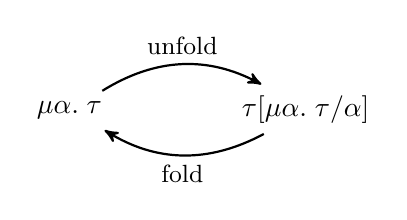
\begin{tikzpicture}[->,>=stealth',shorten >=1pt,auto,node distance=3cm,
  thick,main node/.style={rectangle}]

  \node[main node] (1) {$\mu\alpha.\; \tau$};
  \node[main node] (2) [right of=1] {$\tau[\mu \alpha. \; \tau / \alpha]$};

  \path[every node/.style={font=\sffamily\small}]
    (1) edge [bend left] node [above] {$\unfold$} (2)
    (2) edge [bend left] node [below] {$\fold$} (1);
\end{tikzpicture}
\]
With recursive types in hand we can now define our tree type:
\[
  tree \eqdef \mu \alpha. \; 1 + (int \times \alpha \times \alpha)
\]
When we want to work with this, we would like to be able to get under the $\mu$. Say we have $e : tree$ that is an expression $e$ with type $tree$, then we want to be able to say whether it is a leaf or a node. To do so we unfold the type to get the type where $\alpha$ has been substituted with the definition of $tree$ and the outer $\mu\alpha.$ has been removed. With the outer $\mu\alpha.$ gone we can match on the sum type to find out whether it is a leaf or a node. When we are done working with the type we can fold it back to the original tree type.
\[
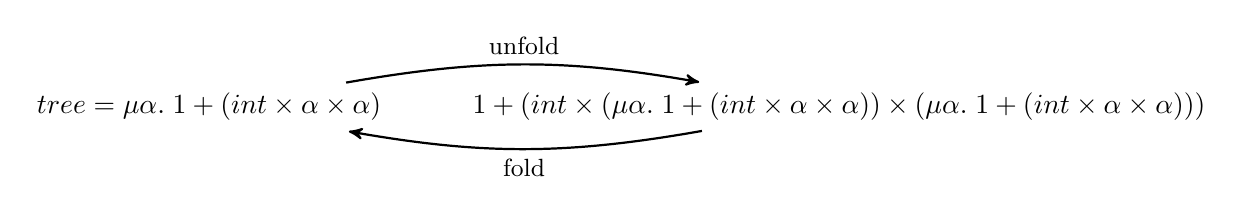
\begin{tikzpicture}[->,>=stealth',shorten >=1pt,auto,node distance=3cm,
  thick,main node/.style={rectangle}]

  \node[main node] (1) {$tree=\mu\alpha.\; 1+(int \times \alpha \times \alpha)$};
  \node[main node] (2) [right of=1,xshift=5cm] {$1+(int \times (\mu\alpha.\; 1+(int \times \alpha \times \alpha)) \times (\mu\alpha.\; 1+(int \times \alpha \times \alpha)))$};

  \path[every node/.style={font=\sffamily\small}]
    (1) edge [bend left=10] node [above] {$\unfold$} (2)
    (2) edge [bend left=10] node [below] {$\fold$} (1);
\end{tikzpicture}
\]
This kind of recursive types is called iso-recursive types, because there is an isomorphism between a $\mu\alpha. \; \tau$ and its unfolding $\tau[\mu\alpha.\; \tau / \alpha]$. 

\subsection*{Simply typed lambda calculus extended with $\mu$}
STLC extended with recursive types is defined as follows:
\begin{align*}
  \tau &::= \dots \vbar \mu \alpha. \; \tau \\
  e    &::= \dots \vbar \fold \; e \vbar \unfold \; e \\
  v    &::= \dots \vbar \fold \; v\\
  E    &::= \dots \vbar \fold \; E \vbar \; \unfold \; E
\end{align*}
\[
\unfold \; (\fold \; v) \evalto v
\]
\[
\TFold \hspace{2cm} \TUnfold
\]
With this we could define the type of an integer list as:
\[
int\; list \eqdef \mu\alpha.\; 1 + (int \times \alpha)
\]
%TODO: Typing omega
\begin{comment}
\[
  \Omega = (\tlabs{x}{\mu\alpha.\; \tarrow{\alpha}{\tau}}{(\unfold \; x) \; x}) 
\]
\end{comment}

\subsection*{Step-indexing, logical relations for recursive types}
In a naive first attempt to make the value interpretation we could write something like
\[
  \vpred{\mu\alpha. \; \tau} = \{\fold \; v \vbar \unfold \; (\fold \; v) \in \epred{\sub{\tau}{\mu\alpha.\;\tau}{\alpha}} \}
\]
We can simplify this slightly; first we use the fact that $\unfold \; (\fold \; v)$ reduces to $v$. Next, we use the fact that $v$ must be a value and the fact that we want $v$ to be in the expression interpretation of $\tau[\mu \alpha. \; \tau / \alpha]$. By unfolding the definition of the expression interpretation we conclude that it suffices to require $v$ to be in the value interpretation of the same type. We then end up with the following definition:
\[
  \vpred{\mu\alpha. \; \tau} = \{\fold \; v \vbar v \in \vpred{\sub{\tau}{\mu\alpha.\;\tau}{\alpha}} \}
\]
This gives us a well-foundedness issue. The value interpretation is defined by induction on the type, but $\sub{\tau}{\mu\alpha.\;\tau}{\alpha}$ is not a structurally smaller type than $\mu\alpha. \; \tau$. 

To solve this issue we index the interpretation by a natural number, $k$, which we write as follows:
\[
  \vpres{\tau} = \{v \vbar \dots \}
\]
Hence, $v \in \vpres{\tau}$ is read as ``$v$ belongs to the interpretation of $\tau$ for $k$ steps.'' We interpret this in the following way: given a value that we run run for $k$ or fewer steps (as in the value is used in some program context for fewer than $k$ steps) then we will never notice that it does not have type $\tau$. If we use the same value in a program context that wants to run for more than $k$ steps, then we might notice that it does not have type $\tau$ which means that we might get stuck. This gives us an approximate guarantee.

We use this as an inductive metric to make our definition well-founded, so we define the interpretation on induction on the step-index followed by an inner induction on the type structure. Let us start by adding the step-index to our existing value interpretation:
\begin{align*}
  \vpres{bool} &= \{\true,\false\} \\
  \vpres{\tarrow{\tau_1}{\tau_2}} &= \{\tlabs{x}{\tau_1}{e} \vbar \forall j \leq k. \; \forall v \in \vpres[j]{\tau_1}. \; \sub{e}{v}{x} \in \epres[j]{\tau_2} \}
\end{align*}
$\true$ and $\false$ are in the value interpretation of $bool$ for any $k$, so $\true$ and $\false$ will for any $k$ look like it has type $bool$. To illustrate how to understand the value interpretation of $\tarrow{\tau_1}{\tau_2}$ please consider the following time line:  \\
\begin{center}
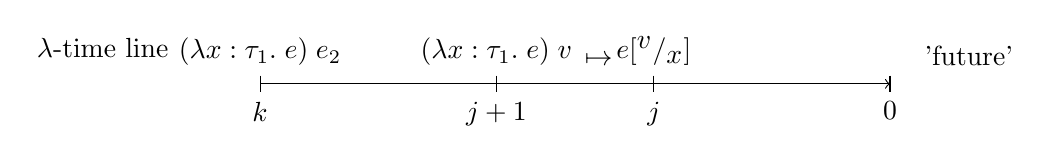
\begin{tikzpicture}
    % draw horizontal line   
    \draw[->] (0,0) -- (8,0);

    % draw vertical lines
    \foreach \x in {0,3,5,8}
      \draw (\x cm,3pt) -- (\x cm,-3pt);

    % draw nodes
    \draw (-2,0) node[below=3pt] {  } node[above=6pt] {$\lambda$-time line};
    \draw (0,0) node[below=3pt] {$k$} node[above=3pt] {$(\tlabs{x}{\tau_1}{e}) \; e_2$};
    \draw (3,0) node[below=3pt] {$ j+1 $} node[above=3pt] {$(\tlabs{x}{\tau_1}{e})\; v $};
    \draw (4.3,0) node[below=3pt] {$   $} node[above=3pt] {$ \evalto $};    
    \draw (5,0) node[below=3pt] {$ j $} node[above=3pt] {$ \sub{e}{v}{x} $};
    \draw (8,0) node[below=3pt] {$ 0 $} node[above=3pt] {$  $};
    \draw (9,0) node[below=3pt] {$   $} node[above=3pt] { 'future' };
  \end{tikzpicture}
\end{center}
Here we start at index $k$ and as we run the program we use up steps until we at some point reach 0 and run out of steps. At step $k$ we are looking at a lambda. A lambda is used by applying it, but it is not certain that the application will happen right away. We only do a $\beta$-reduction when we try to apply a lambda to a value, but we might be looking at a context where we want to apply the lambda to an expressions, i.e.\ $(\tlabs{x}{\tau_1}{e})\; e_2$. We might use a bunch of steps to reduce $e_2$ down to a value, but we cannot say how many. So say that sometime in the future have fully evaluated $e_2$ to $v$ and say that we have $j+1$ steps left at this time, then we can do the $\beta$ reduction which gives us $\sub{e}{v}{x}$ at step $j$. % If we ever hit 0 steps, then all bets are off. the value can have any type.

We can now define the value interpretation of $\mu\alpha. \; \tau$:
\[
  \vpres{\mu\alpha.\; \tau} = \{\fold \; v \vbar \forall j < k. \; v \in \vpres[j]{\sub{\tau}{\mu\alpha.\;\tau}{\alpha}} \}
\]
This definition is like the one we previously proposed, but with a step-index. This definition is well-founded because $j$ is required to be \emph{strictly} less than $k$ and as we define the interpretation on induction over the step-index this is indeed well founded. We do not define a value interpretation for type variables $\alpha$, as we have no polymorphism yet. The only place we have a type variable at the moment is in $\mu\alpha. \; \tau$, but in the interpretation we immediately close off the $\tau$ under the $\mu$, so we will never encounter a free type variable.

Finally, we define the expression interpretation:
\[
  \epres{\tau} = \{e \vbar \forall j < k. \; \forall e'. \; e \evaltos[j] e' \pand \irred(e') \; \implies \; e' \in \vpres[k-j]{\tau}\}
\]
To illustrate what is going on here consider the following time line: \\
\begin{center}
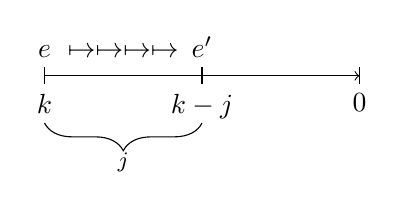
\begin{tikzpicture}
    % draw horizontal line   
    \draw[->] (0,0) -- (4,0);

    % draw vertical lines
    \foreach \x in {0,2,4}
      \draw (\x cm,3pt) -- (\x cm,-3pt);

    % draw nodes
    \draw (0,0) node[below=3pt] {$k$} node[above=3pt] {$e$};
    \draw (1,0) node[below=3pt] {$ $} node[above=3pt] {$\evalto \evalto \evalto \evalto$};
    \draw (2,0) node[below=3pt] {$k-j$} node[above=3pt] {$e'$};
    \draw (4,0) node[below=3pt] {$0$} node[above=3pt] {$  $};

    % brace
    \draw [decorate,decoration={brace,amplitude=10pt,mirror}]
    (0,-0.6) -- (2,-0.6) node [black,midway,yshift=-0.5cm] 
          {\footnotesize $j$};
\end{tikzpicture}
\end{center}
We start with an expression $e$, then we take $j$ steps and get to expression $e'$. At this point if $e'$ is irreducible, then we want it to belong to the value interpretation of $\tau$ for $k-j$ steps. We use a strict inequality because we do not want to hit 0 steps. If we hit 0 steps, then all bets are off.%TODO: why are all bets off?

We also need to lift the interpretation of type environments to step-indexing:
\begin{align*}
  \gpres{\mtenv} & = \{\emptyset \} \\
  \gpres{\Gamma, x : \tau} & = \{ \gamma[x \mapsto v] \vbar \gamma \in \gpres{\Gamma} \pand v \in \vpres{\tau} \}
\end{align*}
Finally we are in a position to lift the definition of semantic type safety to one with step-indexing.
\[
  \Gamma \models e : \tau \eqdef \forall k \geq 0. \; \forall \gamma \in \gpres{\Gamma} \; \implies \gamma(e) \in \epres{\tau}
\]
To actually prove type safety we do it in two steps. First we state and prove the fundamental theorem:
\begin{stlcmufundprop}[Fundamental property] ~\\
  If $\Gamma \vdash e : \tau$ then $\Gamma \models e : \tau$.
\end{stlcmufundprop}
When we have proven the fundamental theorem we prove that it entails type safety.
\[
\circled{b} \quad \mtenv \models e : \tau \implies \safe(e)
\]
Thanks to the way we defined the logical predicate this second step should be trivial to prove.

To actually prove the fundamental theorem, which is the challenging part, we need to prove a monotonicity lemma:
\begin{monotonicity}[Monotonicity] ~\\
  If $v\in \vpres{\tau}$ and $j \leq k$  then $v \in \vpres[j]{\tau}$.
\end{monotonicity}
\begin{proof}
The proof is by case on $\tau$.
\case{$\tau = bool$}
assume $v \in \vpres{bool}$ and $j \leq k$, we then need to show $v \in \vpres[j]{bool}$. As $v \in \vpres{bool}$ we know that either $v= \true$ or $v=\false$. If we assume $v=\true$, then we immediately get what we want to show, as $\true$ is in $\vpres[j]{bool}$ for any $j$. Likewise for the case $v=\false$.
\case{$\tau = \tarrow{\tau_1}{\tau_2}$}
assume $v \in \vpres{\tarrow{\tau_1}{\tau_2}}$ and $j \leq k$, we then need to show $v \in \vpres[j]{\tarrow{\tau_1}{\tau_2}}$. As $v$ is a member of $\vpres{\tarrow{\tau_1}{\tau_2}}$ we can conclude that $v = \tlabs{x}{\tau_1}{e}$ for some $e$. By definition of $v \in \vpres[j]{\tarrow{\tau_1}{\tau_2}}$ we need to show $\forall i \leq j. \forall v' \in \vpres[i]{\tau_1}.\; \sub{e}{v'}{x} \in \epres[i]{\tau_2}$. Suppose $i \leq j$ and $v' \in \vpres[i]{\tau_1}$, we then need to show $\sub{e}{v'}{x} \in \epres[i]{\tau_2}$.

By assumption we have $v \in \vpres{\tarrow{\tau_1}{\tau_2}}$ which gives us $\forall n \leq k. \; \forall v' \in \vpres[n]{\tau_1}.\; \sub{e}{v'}{x} \in \epres[n]{\tau_2}$. From $j \leq k$ and $i \leq j$ we get $i \leq k$ by transitivity. We use this with $v' \in \vpres[i]{\tau_1}$ to get $\sub{e}{v'}{x} \in \epres[i]{\tau_2}$ which is what we needed to show.
\case{$\tau = \mu \alpha.\; x$}
assume $v \in \vpres{\mu\alpha. \; \tau}$ and $j \leq k$, we then need to show $v \in \vpres[j]{\mu\alpha. \; \tau}$. From $v$'s assumed membership of the value interpretation of $\tau$ for $k$ steps we conclude that there must exist a $v'$ such that $v = \fold \; v'$. If we suppose $i<j$, then we need to show $v' \in \vpres[i]{\subst{\tau}{\mu\alpha.\; \tau}{\alpha}}$. From $i<j$ and $j \leq k$ we can conclude $i < k$ which we use with $\forall n < k.\; v' \in \vpres[n]{\subst{\tau}{\mu\alpha.\; \tau}{\alpha}}$, which we get from $v \in \vpres{\mu\alpha. \; \tau}$, to get $v' \in \vpres[i]{\subst{\tau}{\mu\alpha.\; \tau}{\alpha}}$.
\end{proof}
\begin{comment}
  \begin{lemma}[Substitution]
    Let $e$ be syntactically well-formed term, let $v$ be a closed value and let $\gamma$ be a substitution that map term variables to closed values, and let $x$ be a variable not in the domain of $\gamma$, then
    \[
    \extsub{\gamma}{x}{v}(e) = \subst{\gamma(e)}{x}{v}
    \]
  \end{lemma}
\end{comment}
\begin{proof}[Proof (Fundamental Property)]
Proof by induction over the typing derivation.
\case{\TFold} \\~
We need to show 
\newcommand{\mat}{\ensuremath{\mu\alpha.\tau}}
v\[
  \Gamma \models \fold \; e : \mat
\]
So suppose we have $k \geq 0$ and $\gamma \in \gpres{\mat}$, then we need to show $\gamma(\fold\; e) \in \epres{\mat}$ which amounts to showing $\fold\; \gamma(e) \in \epres{\mat}$.

So suppose that $j<k$ and that $\fold\; \gamma(e) \evaltos[j] e'$ and $\irred(e')$, then we need to show $e' \in \vpres[k-j]{\mat}$. As we have assumed that $\fold\; \gamma(e)$ reduces down to something irreducible and the operational semantics of this language are deterministic we know that $\gamma(e)$ must have evaluated down to something irreducible. We therefore know that $\gamma(e) \evaltos[j_1] e_1$ where $j_1 \leq j$ and $\irred(e_1)$.
Now we use our induction hypothesis:
\newcommand{\tsub}{\ensuremath{\sub{\tau}{\mat}{\alpha}}}
\[
  \Gamma \models e : \tsub
\]
We instantiate this with $k$ and $\gamma \in \gpres{\Gamma}$ to get $\gamma(e) \in \epres{\tsub}$. Which we then can instantiate with $j_1$ and $e_1$ for get $e_1 \in \vpres[k-j_1]{\tsub}$. Now let us take a step back and see what happened: We started with a $\fold\; \gamma(e)$ which took $j_1$ steps to $\fold\; e_1$. We have just shown that this $e_1$ is actually a value as it is in the value interpretation of $\vpres[k-j_1]{\tsub}$. To remind us $e_1$ is a value let us henceforth refer to it as $v_1$. We further know that $\fold\; \gamma(e)$ reduces to $e'$ in $j$ steps and that $e'$ was irreducible. $\fold\; v_1$ is also irreducible as it is a value and as our language is deterministic it must be the case that $e' = \fold\; v_1$ and thus $j = j_1$. Our proof obligation was to show $e' = \fold \; v_1 \in \vpres[k-j]{\mat}$ to show this suppose we have $l < k-j$ (this also gives us $l < k-j_1$ as $j = j_1$). We then need to show $v_1 \in \vpres[l]{\tsub}$, we obtain this result from the monotonicity lemma using $\vpres[k-j_1]{\tsub}$ and $l < k-j_1$.
\end{proof}

The list example from the previous lecture used the sum type. Sums are a straight forward extension of the language. The extension of the value interpretation would be:
\[
  \vpres{\tau_1 + \tau_2} = \{\inl \; v_1 \vbar v_1 \in \vpres{\tau_1}\} \cup 
                            \{\inr \; v_2 \vbar v_2 \in \vpres{\tau_2}\}
\]
We can use $k$ directly or $k$ decremented by one. It depends on whether we want casing to take up a step. Either way the definition is well-founded. 

\subsection*{Exercises}
\begin{enumerate}
\item Do the lambda and application case of the \emph{Fundamental Property} theorem.%Specify in what proof, probably fundemental property
\item Try to prove the \emph{monotonicity} lemma where the definition of the value interpretation has been adjusted with:
\[
\vpres{\tarrow{\tau_1}{\tau_2}} = \{\tlabs{x}{\tau_1}{e} \vbar \; \forall v \in \vpres{\tau_1}. \; \sub{e}{v}{x} \in \epres{\tau_2} \}
\]
This will fail, but it is instructive to see how it fails.
\end{enumerate}
%Recursive types
\section*{Acknowledgments} It is established practice for authors to accept responsibility for any and all mistakes in documents like this. I, however, do not. If
you find anything amiss, please let me know so I can figure out who of the following are to blame: Amal Ahmed, Morten Krogh-Jespersen or Kristoffer Just Andersen.
\end{document}
